\documentclass[12pt,a4paper]{report}

% ==============================================================================
% Institutional Page Geometry (Symmetric margins for balanced page border layout)
% Left margin = 3.0 cm, Right = 3.0 cm, Top = 3.0 cm, Bottom = 3.0 cm
% ==============================================================================
\usepackage[a4paper, left=3.0cm, right=3.0cm, top=3.0cm, bottom=3.0cm]{geometry}

% Standard Typography: Times New Roman 12pt with 1.5 Line Spacing
\usepackage{mathptmx}
\usepackage{setspace}
\onehalfspacing

% Indentation: 5 spaces (~1.5em) for fresh paragraphs
\setlength{\parindent}{1.5em}
\setlength{\parskip}{0.5em}

% Essential Packages
\usepackage{graphicx}
\usepackage{fancyhdr}
\usepackage{titlesec}
\usepackage{booktabs}
\usepackage{tabularx}
\usepackage{array}
\usepackage{longtable}
\usepackage{multirow}
\usepackage{float}
\usepackage{caption}
\usepackage{subcaption}
\usepackage{amssymb}
\usepackage{pifont}
\usepackage{xcolor}
\usepackage{enumitem}

% Page Border on Every Page (matching Geethanjali College template)
\usepackage{tikz}
\usepackage{eso-pic}

\AddToShipoutPictureBG{%
  \begin{tikzpicture}[remember picture, overlay]
    \draw[line width=0.8pt, black]
      ([xshift=24pt, yshift=-24pt]current page.north west)
      rectangle
      ([xshift=-24pt, yshift=24pt]current page.south east);
  \end{tikzpicture}%
}

% Hyperlinks & PDF Metadata
\usepackage[hidelinks, pdftex,
  pdfauthor={G.Himavanth Kumar},
  pdftitle={Internship Report - ShopSphere: Full-Stack E-Commerce Management System},
  pdfsubject={B.Tech Internship Report},
  pdfkeywords={Full Stack, React, Spring Boot, MySQL, Razorpay, JWT}]{hyperref}

% Heading Formatting: No underlines, NO colons in headings
% Main Heading: 16pt Bold Times New Roman
% Sub Heading: 14pt Bold Times New Roman
% Sub-sub Heading: 12pt Bold Times New Roman
\titleformat{\chapter}[hang]
  {\normalfont\fontsize{16}{20}\bfseries}{\thechapter}{1em}{}
\titlespacing*{\chapter}{0pt}{-10pt}{18pt}

\titleformat{\section}
  {\normalfont\fontsize{14}{18}\bfseries}{\thesection}{1em}{}
\titlespacing*{\section}{0pt}{12pt}{6pt}

\titleformat{\subsection}
  {\normalfont\fontsize{12}{16}\bfseries}{\thesubsection}{1em}{}
\titlespacing*{\subsection}{0pt}{10pt}{4pt}

% Running Header & Footer Configuration (Matching Demo PDF: Institutional Footer at bottom)
\pagestyle{fancy}
\fancyhf{}
\fancyfoot[L]{\fontsize{10}{12}\selectfont Internship Report}
\fancyfoot[C]{\fontsize{10}{12}\selectfont Department of CSE-AI\&ML}
\fancyfoot[R]{\fontsize{10}{12}\selectfont 2026-27}
\renewcommand{\headrulewidth}{0pt}
\renewcommand{\footrulewidth}{0pt}

% Plain page style (used for chapter first pages)
\fancypagestyle{plain}{
  \fancyhf{}
  \fancyfoot[L]{\fontsize{10}{12}\selectfont Internship Report}
  \fancyfoot[C]{\fontsize{10}{12}\selectfont Department of CSE-AI\&ML}
  \fancyfoot[R]{\fontsize{10}{12}\selectfont 2026-27}
  \renewcommand{\headrulewidth}{0pt}
  \renewcommand{\footrulewidth}{0pt}
}

% Path for Images
\graphicspath{{images/}}

% Custom Checkmark commands
\newcommand{\cmark}{\ding{51}}
\newcommand{\xmark}{\ding{55}}

\begin{document}

% ------------------------------------------------------------------------------
% PRELIMINARY FRONTMATTER (Roman Numerals: i, ii, iii...)
% ------------------------------------------------------------------------------
\pagenumbering{roman}

% 1. Title Page (Cover)
\begin{titlepage}
\begin{center}
    {\large An}\\[0.2cm]
    {\large \textbf{Internship Report on}}\\[0.6cm]
    
    {\fontsize{18}{22}\selectfont \textbf{SHOPSPHERE: FULL-STACK E-COMMERCE MANAGEMENT SYSTEM}}\\[1.0cm]
    
    {\large \textit{Submitted}}\\[0.2cm]
    {\large \textit{in partial fulfillment of the requirements for the award of the degree of}}\\[0.6cm]
    
    {\fontsize{15}{18}\selectfont \textbf{BACHELOR OF TECHNOLOGY}}\\[0.3cm]
    {\large in}\\[0.3cm]
    {\fontsize{14}{17}\selectfont \textbf{CSE-Artificial Intelligence and Machine Learning}}\\[0.8cm]
    
    {\large By}\\[0.4cm]
    {\fontsize{15}{18}\selectfont \textbf{G.Himavanth Kumar}}\\[0.2cm]
    {\fontsize{14}{17}\selectfont \textbf{24R11A6617}}\\[1.0cm]
    
    % College Emblem
    
\includegraphics[width=2.8cm, height=2.8cm, keepaspectratio]{college_logo.jpeg}\\[0.6cm]
    
    {\fontsize{16}{20}\selectfont \textbf{\textcolor{green!60!black}{Department of CSE-Artificial Intelligence and Machine Learning}}}\\[0.25cm]
    {\fontsize{20}{24}\selectfont \textbf{\textcolor{blue!70!black}{Geethanjali College of Engineering and Technology}}}\\[0.2cm]
    {\fontsize{12}{15}\selectfont \textbf{\textcolor{red!80!black}{(UGC AUTONOMOUS INSTITUTION)}}}\\[0.2cm]
    {\fontsize{11}{14}\selectfont \textcolor{blue!60!black}{(Affiliated to J.N.T.U.H, Approved by AICTE, New Delhi)}}\\[0.1cm]
    {\fontsize{11}{14}\selectfont Cheeryal (V), Keesara (M), Medchal Dist. - 501 301.}\\[0.6cm]
    
    {\fontsize{14}{17}\selectfont \textbf{August - 2026}}
    
    \vfill
    {\small \textbf{Internship Report} \hfill \textbf{Department of CSE-AI\&ML} \hfill \textbf{2026-27}}
\end{center}
\end{titlepage}


% 2. College Certificate
\newpage
\thispagestyle{fancy}
\begin{center}
    {\fontsize{20}{24}\selectfont \textbf{\textcolor{red!80!black}{Geethanjali College of Engineering \& Technology}}}\\[0.15cm]
    {\large \textbf{(UGC Autonomous)}}\\[0.1cm]
    {\small (Affiliated to JNTUH, Approved by AICTE, New Delhi)}\\[0.1cm]
    {\small Cheeryal (V), Keesara (M), Medchal Dist. - 501 301.}\\[0.4cm]
    
    {\fontsize{13}{16}\selectfont \textbf{\textcolor{blue!80!black}{Department of CSE-Artificial Intelligence and Machine Learning}}}\\[0.5cm]
    
    
\includegraphics[width=2.4cm, height=2.4cm, keepaspectratio]{college_logo.jpeg}\\[0.2cm]
    {\textbf{Geethanjali}}\\[0.5cm]
    
    {\fontsize{16}{20}\selectfont \textbf{\textit{\textcolor{orange!80!black}{\underline{CERTIFICATE}}}}}\\[0.8cm]
\end{center}

\noindent This is to certify that the internship report titled \textbf{``ShopSphere: Full-Stack E-Commerce Management System''} being submitted by \textbf{G.Himavanth Kumar}, bearing roll number \textbf{24R11A6617}, in partial fulfillment of the requirements for the award of the Degree of Bachelor of Technology in \textbf{``CSE-Artificial Intelligence and Machine Learning''} from \textbf{Jawaharlal Nehru Technological University, Hyderabad} during the academic year 2026--2027.

\vspace{1.8cm}

\noindent
\begin{tabular}{p{7.0cm}p{7.0cm}}
    \textbf{Internship Supervisor} & \textbf{Internship Coordinator} \\[0.2cm]
    \textbf{Mrs. P Swathi} & \textbf{Mr. Vedavyas Gurla} \\
    (Asst. Professor, CSE-AI\&ML) & (Assoc. Professor, CSE-AI\&ML) \\[2.0cm]
\end{tabular}

\begin{center}
    \textbf{Dr. L. Venkateswarlu}\\
    (Professor \& HoD, CSE-AI\&ML)
\end{center}

\vspace{1.2cm}

\noindent
\textbf{Examiner}\\
Signature:\ \dotfill\\
Name:\ \dotfill\\
Designation:\ \dotfill


% 3. Company Certificate (Codec Technologies Pvt. Ltd.)
\newpage
\thispagestyle{fancy}

\begin{center}
    {\fontsize{14}{17}\selectfont \textbf{INTERNSHIP CERTIFICATE FROM ORGANIZATION WITH LETTERHEAD}}\\[0.8cm]
    
    \fbox{%
        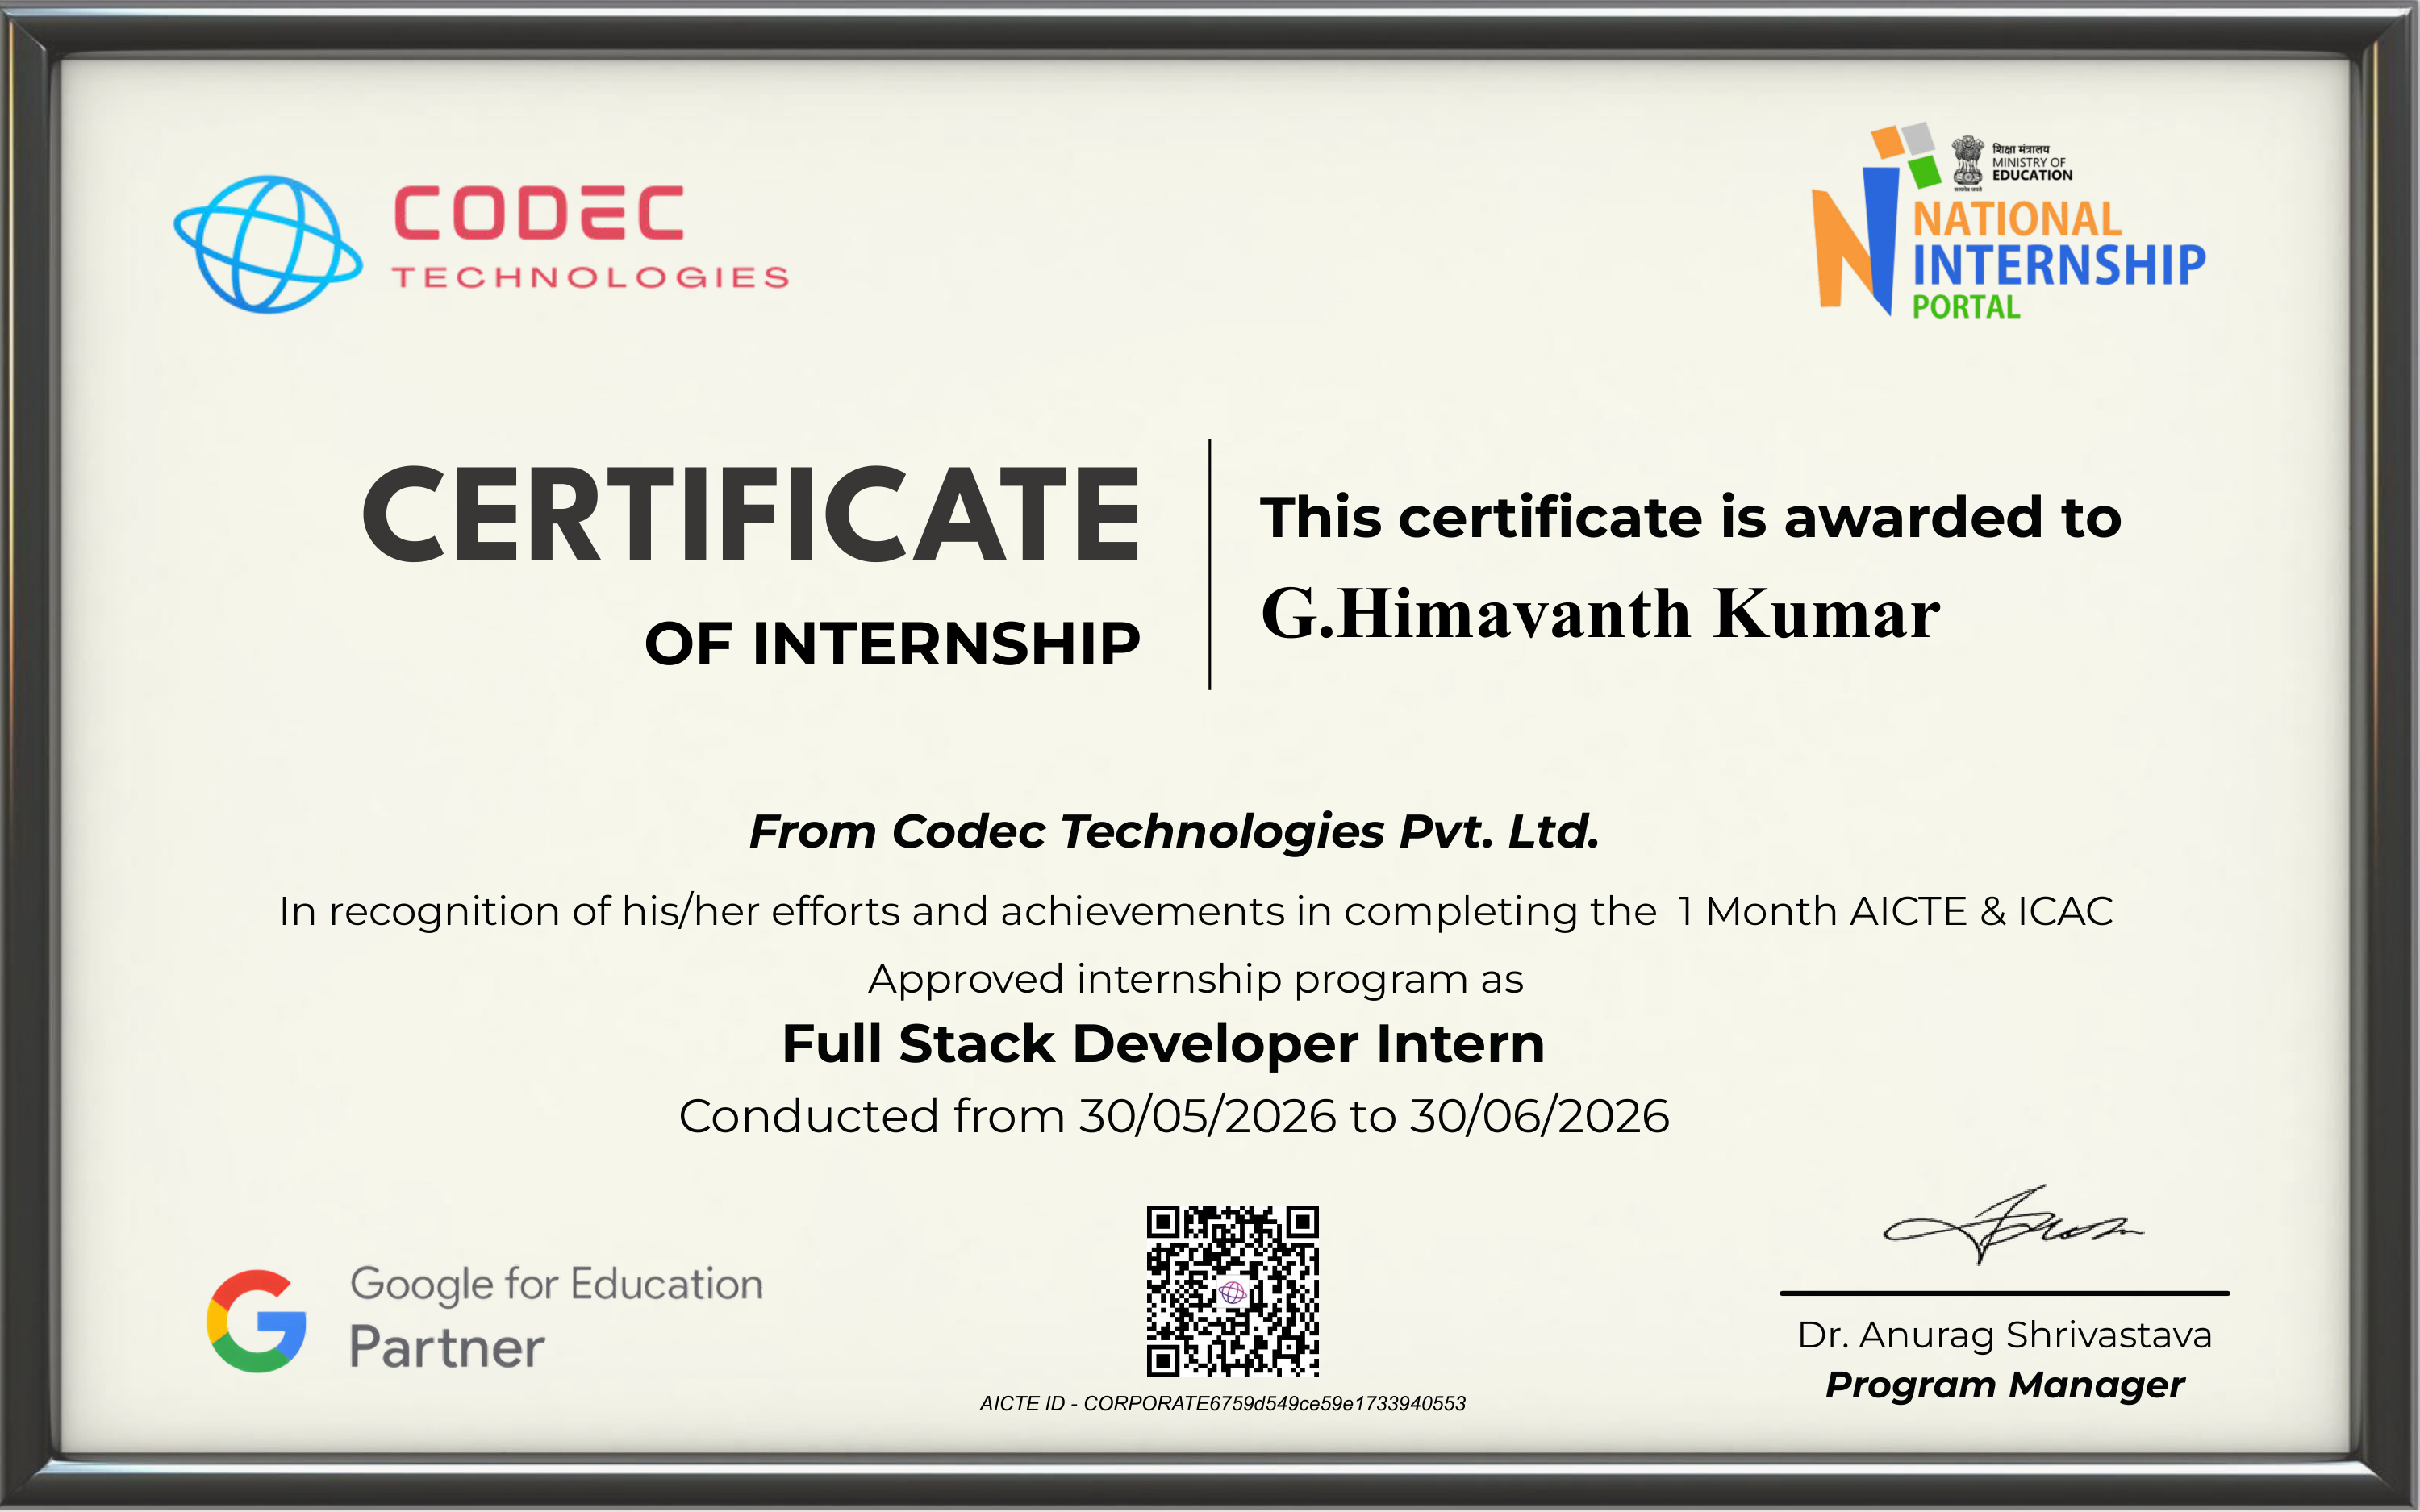
\includegraphics[width=0.96\textwidth, height=0.72\textheight, keepaspectratio]{codec_internship_certificate.png}%
    }\\[0.8cm]
\end{center}

\noindent
\begin{minipage}{0.96\textwidth}
    \small
    \textbf{Organization:} Codec Technologies Pvt. Ltd.\\
    \textbf{Program:} 1 Month AICTE \& ICAC Approved Internship Program\\
    \textbf{Designation:} Full Stack Developer Intern\\
    \textbf{Tenure:} 30/05/2026 to 30/06/2026\\
    \textbf{AICTE ID:} CORPORATE6759d549ce59e1733940553\\
    \textbf{Program Manager:} Dr. Anurag Shrivastava
\end{minipage}


% 4. Candidate Declaration
\newpage
\thispagestyle{fancy}
\begin{center}
    {\fontsize{20}{24}\selectfont \textbf{\textcolor{red!80!black}{Geethanjali College of Engineering \& Technology}}}\\[0.15cm]
    {\large \textbf{(UGC Autonomous)}}\\[0.1cm]
    {\small (Affiliated to JNTUH, Approved by AICTE, New Delhi)}\\[0.1cm]
    {\small Cheeryal (V), Keesara (M), Medchal Dist. - 501 301.}\\[0.4cm]
    
    {\fontsize{13}{16}\selectfont \textbf{\textcolor{blue!80!black}{Department of CSE-Artificial Intelligence and Machine Learning}}}\\[0.5cm]
    
    
\includegraphics[width=2.2cm, height=2.2cm, keepaspectratio]{college_logo.jpeg}\\[0.2cm]
    {\textbf{Geethanjali}}\\[0.6cm]
    
    {\fontsize{15}{18}\selectfont \textbf{\textcolor{orange!80!black}{\underline{DECLARATION BY THE CANDIDATE}}}}\\[1.0cm]
\end{center}

\noindent I, \textbf{G.Himavanth Kumar}, bearing Roll No. \textbf{24R11A6617}, hereby declare that the Internship Report entitled \textbf{``ShopSphere: Full-Stack E-Commerce Management System''} is submitted in partial fulfillment of the requirements for the award of the degree of \textbf{Bachelor of Technology in CSE-Artificial Intelligence and Machine Learning}.

\vspace{0.8cm}

\noindent This is a record of bonafide work carried out by me in \textbf{Codec Technologies Pvt. Ltd.} and the results embodied in this internship have not been reproduced or copied from any source. The results embodied in this Internship Report have not been submitted to any other University or Institute.

\vspace{3.0cm}

\begin{flushright}
    \textbf{Signature of Student}\\[0.3cm]
    \textbf{G.Himavanth Kumar}\\
    Roll No: \textbf{24R11A6617}
\end{flushright}


% 5. Acknowledgement
\newpage
\thispagestyle{fancy}
\begin{center}
    {\fontsize{16}{20}\selectfont \textbf{ACKNOWLEDGEMENT}}\\[1.0cm]
\end{center}

\noindent I would like to express my heartfelt gratitude to everyone who played a role in the successful completion of this project. My deepest thanks go to our Director, \textbf{Dr. Uday Kumar Susarla}, and our college Principal, \textbf{Dr. K. Sagar}, for providing the essential resources and unwavering support for this endeavor. I am profoundly grateful to the Professor \& Dean - School of CS and Informatics, \textbf{Dr. V. Madhusudan Rao}, and our Head of the Department, \textbf{Dr. L. Venkateswarlu}, for his invaluable guidance and encouragement throughout the internship project.

\vspace{0.8cm}

\noindent I would like to extend my heartfelt gratitude to our beloved faculty as Internship supervisor, \textbf{Mrs. P Swathi}, whose invaluable expertise and guidance were instrumental to our success. I am also sincerely appreciative of our Internship Coordinator, \textbf{Mr. Vedavyas Gurla}, for the unwavering support and encouragement throughout this period. Additionally, I am deeply grateful to \textbf{Codec Technologies Pvt. Ltd.} and my internship guide, \textbf{Dr. Anurag Shrivastava (Program Manager)}, for this incredible opportunity, continuous training, and invaluable guidance throughout my journey. Thank you all for your significant contributions to my learning and growth.

\vspace{2.5cm}

\begin{flushright}
    \textbf{G.Himavanth Kumar}\\
    Roll No: \textbf{24R11A6617}\\
    B.Tech (CSE-AI\&ML)\\
    Geethanjali College of Engineering and Technology
\end{flushright}


% 6. Introduction about Internship Organization
\newpage
\thispagestyle{fancy}
\begin{center}
    {\fontsize{16}{20}\selectfont \textbf{INTRODUCTION ABOUT INTERNSHIP ORGANIZATION}}\\[0.8cm]
\end{center}

\noindent \textbf{Codec Technologies Pvt. Ltd.} is a premier technology solutions provider and digital consulting enterprise specializing in cutting-edge software architecture, cloud platforms, full-stack enterprise development, and artificial intelligence-driven products. Headquartered in India, the organization operates as an accredited technology provider partnered with leading academic and industry bodies, including the \textbf{All India Council for Technical Education (AICTE)} and the \textbf{National Internship Portal (NIP)}. Codec Technologies is also recognized as an official \textbf{Google for Education Partner}, emphasizing its dedication to technical upskilling, experiential engineering, and digital transformation.

\vspace{0.4cm}
\noindent \textbf{1. Vision and Mission}
\begin{itemize}[leftmargin=2.0em]
    \item \textbf{Vision:} To empower modern global businesses through scalable, resilient, and human-centric software solutions while cultivating world-class software engineering talent through rigorous hands-on technical programs.
    \item \textbf{Mission:} To deliver enterprise-grade digital products across e-commerce, cloud computing, and intelligent data systems by leveraging modern architectures such as microservices, reactive frontend frameworks, and cloud-native databases.
\end{itemize}

\vspace{0.4cm}
\noindent \textbf{2. Core Competencies and Engineering Domains}
Codec Technologies provides engineering services across several multidisciplinary technology verticals:
\begin{enumerate}[leftmargin=2.0em]
    \item \textbf{Enterprise Full-Stack Web Development:} Designing robust decoupled systems utilizing React.js, Angular, Next.js, Java Spring Boot, Node.js, and Python FastAPI.
    \item \textbf{Cloud Infrastructure and DevOps:} Deploying resilient containerized architectures using Docker, Kubernetes, AWS, Microsoft Azure, and CI/CD pipelines.
    \item \textbf{Data Engineering and Artificial Intelligence:} Developing predictive analytics models, real-time analytics dashboards, and natural language processing pipelines.
    \item \textbf{Payment Systems and Financial Cryptography:} Integrating secure payment gateways (Razorpay, Stripe) with cryptographic signature validation (HMAC-SHA256) and PCI-DSS compliance.
\end{enumerate}

\vspace{0.4cm}
\noindent \textbf{3. The AICTE-Approved Full Stack Developer Internship Program}
The 1-month intensive internship program (conducted under Corporate AICTE ID: \texttt{CORPORATE6759d549ce59e1733940553}) was designed to transition undergraduate engineering scholars into production-capable full-stack developers. Under the mentorship of Program Manager \textbf{Dr. Anurag Shrivastava}, interns are immersed in production-level version control, agile sprint planning, RESTful API design, database normalization, stateless authentication with Spring Security and JWT, and responsive client-side development. Interns are assigned capstone enterprise assignments—exemplified by the \textbf{ShopSphere E-Commerce Management System}—demanding rigorous software engineering discipline, comprehensive automated testing, and industry-standard documentation.


% 7. 4-Week Training Schedule
\newpage
\thispagestyle{fancy}
\begin{center}
    {\fontsize{16}{20}\selectfont \textbf{TRAINING SCHEDULE}}\\[0.6cm]
\end{center}

\noindent The 1-Month Full Stack Developer Internship at \textbf{Codec Technologies Pvt. Ltd.} was conducted from \textbf{30/05/2026 to 30/06/2026}. The training was organized into four progressive engineering modules, combining theoretical architecture with hands-on implementation of the \textbf{ShopSphere} capstone platform.

\vspace{0.4cm}

\begin{table}[H]
\centering
\fontsize{10.5}{14}\selectfont
\begin{tabularx}{\textwidth}{|c|p{3.2cm}|X|p{2.8cm}|}
\hline
\textbf{Week} & \textbf{Duration} & \textbf{Modules and Practical Topics Covered} & \textbf{Key Deliverables} \\
\hline
\textbf{Week 1} & 
30/05/2026 -- 06/06/2026 & 
\textbf{Enterprise Architecture \& Database Engineering}:
\begin{itemize}[leftmargin=1.2em, topsep=2pt, parsep=0pt]
    \item Java 22 features, Git branching \& collaboration.
    \item Spring Boot 3.3 project scaffolding and Maven build.
    \item RESTful architectural constraints and DTO pattern.
    \item MySQL 8 relational modeling (19 tables in 3NF).
\end{itemize} & 
Initial schema script (\texttt{schema.sql}), seed data (\texttt{data.sql}), and Maven project baseline. \\
\hline
\textbf{Week 2} & 
07/06/2026 -- 14/06/2026 & 
\textbf{Persistence Layer \& Security Architecture}:
\begin{itemize}[leftmargin=1.2em, topsep=2pt, parsep=0pt]
    \item Spring Data JPA and Hibernate 6 ORM entity mapping.
    \item Spring Security 6 stateless filter chain.
    \item BCrypt password hashing (10 salt rounds).
    \item HMAC-SHA256 JWT token generation and validation.
    \item Role-Based Access Control (\texttt{ROLE\_CUSTOMER}, \texttt{ROLE\_ADMIN}).
\end{itemize} & 
Auth REST controllers, JWT filter, repository layer, and authenticated endpoints. \\
\hline
\textbf{Week 3} & 
15/06/2026 -- 22/06/2026 & 
\textbf{Modern Reactive Frontend Engineering}:
\begin{itemize}[leftmargin=1.2em, topsep=2pt, parsep=0pt]
    \item React 18 component architecture and Vite bundler.
    \item Redux Toolkit for global auth, cart, and wishlist state.
    \item React Router v6 public and protected role guards.
    \item Axios HTTP client with automated Bearer token injection.
    \item Storefront UI, multi-faceted filtering, and dynamic cart.
\end{itemize} & 
Responsive React client, category pills, price slider, and persistent cart module. \\
\hline
\textbf{Week 4} & 
23/06/2026 -- 30/06/2026 & 
\textbf{Payment Gateway, Business Rules \& Analytics}:
\begin{itemize}[leftmargin=1.2em, topsep=2pt, parsep=0pt]
    \item Razorpay checkout integration and server HMAC check.
    \item Verified purchase review gate implementation.
    \item Concurrency control with atomic inventory decrement.
    \item Admin analytics dashboard with real-time sales KPIs.
    \item End-to-end integration testing and report synthesis.
\end{itemize} & 
Verified payment flow, admin management portal, full documentation, and project sign-off. \\
\hline
\end{tabularx}
\caption{Detailed 4-Week Internship Training Schedule (Codec Technologies)}
\label{tab:training_schedule}
\end{table}


% 8. Abstract
\newpage
\thispagestyle{fancy}
\begin{center}
    {\fontsize{16}{20}\selectfont \textbf{ABSTRACT}}\\[0.8cm]
\end{center}

\noindent Modern digital commerce platforms demand high responsiveness, resilient transactional integrity, robust data security, and comprehensive administrative observability. Conventional monolithic implementations frequently suffer from tight architectural coupling, susceptibility to inventory race conditions, inconsistent cart calculations, and fragile client-side payment handling. To address these industrial challenges, this internship project introduces \textbf{ShopSphere}—an enterprise-grade, full-stack e-commerce management system engineered using a decoupled 3-tier architecture.

\vspace{0.3cm}

\noindent The presentation layer is constructed with \textbf{React.js 18} and \textbf{Vite}, incorporating \textbf{Redux Toolkit} for predictable state synchronization across carts, wishlists, and authenticated sessions. The frontend features a responsive storefront, dynamic multi-faceted filtering (category, brand, rating, and dynamic price sliders), an instant live search engine, and an itemized shopping cart with automated 18\% GST and shipping calculations. The application backend is built with \textbf{Java 22} and \textbf{Spring Boot 3.3.4}, exposing secure RESTful endpoints governed by \textbf{Spring Security 6} and stateless \textbf{JSON Web Token (JWT)} authentication with \textbf{BCrypt} password salting. Role-Based Access Control (RBAC) strictly separates customer operations from privileged administrative endpoints.

\vspace{0.3cm}

\noindent Data persistence is powered by \textbf{MySQL 8}, architected into 19 relational tables normalized to \textbf{Third Normal Form (3NF)}. The schema incorporates explicit foreign key cascade constraints, indexed query paths, and historical price snapshotting on line items to guarantee financial auditability. Real-world business logic is enforced through declarative Spring \texttt{@Transactional} boundaries:
\begin{enumerate}[leftmargin=2.0em, topsep=2pt, parsep=0pt]
    \item \textbf{Verified Purchase Review Gate:} Customers are restricted from reviewing products unless they possess a confirmed and \texttt{DELIVERED} order for that specific item.
    \item \textbf{Atomic Inventory Decrement:} Prevents overselling race conditions under concurrent checkouts using atomic SQL updates and low-stock sentinel alerts.
    \item \textbf{Cryptographic Payment Integrity:} Integrates the \textbf{Razorpay} payment gateway with server-side \textbf{HMAC-SHA256} signature verification, guaranteeing that order fulfillment occurs only upon authenticated payment validation.
\end{enumerate}

\vspace{0.3cm}

\noindent An integrated administrative portal provides executive business intelligence, featuring real-time KPI metrics, monthly sales trend visualizations, order status lifecycle management (\texttt{PLACED} to \texttt{DELIVERED}), and full catalog CRUD capabilities. The complete platform was successfully developed, tested, and validated during the internship at \textbf{Codec Technologies Pvt. Ltd.}, fulfilling all industrial objectives and institutional evaluation benchmarks.


% 9. Table of Contents & Lists
\tableofcontents
\newpage

\listoffigures
\newpage

\listoftables
\newpage

% List of Symbols & Abbreviations
\newpage
\thispagestyle{fancy}
\begin{center}
    {\fontsize{16}{20}\selectfont \textbf{LIST OF SYMBOLS \& ABBREVIATIONS}}\\[0.8cm]
\end{center}

\begin{table}[H]
\centering
\begin{tabularx}{\textwidth}{p{3.2cm}X}
\toprule
\textbf{Abbreviation} & \textbf{Full Expansion / Description} \\
\midrule
\textbf{3NF} & Third Normal Form (Relational Database Normalization) \\
\textbf{ACID} & Atomicity, Consistency, Isolation, Durability \\
\textbf{AICTE} & All India Council for Technical Education \\
\textbf{API} & Application Programming Interface \\
\textbf{B.Tech} & Bachelor of Technology \\
\textbf{CDN} & Content Delivery Network \\
\textbf{COD} & Cash on Delivery \\
\textbf{CORS} & Cross-Origin Resource Sharing \\
\textbf{CRUD} & Create, Read, Update, Delete \\
\textbf{CSE} & Computer Science and Engineering \\
\textbf{CSS} & Cascading Style Sheets \\
\textbf{DAO} & Data Access Object \\
\textbf{DOM} & Document Object Model \\
\textbf{DTO} & Data Transfer Object \\
\textbf{ER} & Entity-Relationship \\
\textbf{FK} & Foreign Key \\
\textbf{GST} & Goods and Services Tax \\
\textbf{HMAC} & Hash-based Message Authentication Code \\
\textbf{HoD} & Head of the Department \\
\textbf{HTML} & HyperText Markup Language \\
\textbf{HTTP / HTTPS} & HyperText Transfer Protocol / Secure \\
\textbf{JPA} & Java Persistence API \\
\textbf{JSON} & JavaScript Object Notation \\
\textbf{JWT} & JSON Web Token (RFC 7519) \\
\textbf{KPI} & Key Performance Indicator \\
\textbf{MVC} & Model-View-Controller \\
\textbf{ORM} & Object-Relational Mapping \\
\textbf{PCI-DSS} & Payment Card Industry Data Security Standard \\
\textbf{PK} & Primary Key \\
\textbf{PO} & Program Outcome \\
\textbf{PSO} & Program Specific Outcome \\
\textbf{RBAC} & Role-Based Access Control \\
\textbf{REST} & Representational State Transfer \\
\textbf{SHA-256} & Secure Hash Algorithm 256-bit \\
\textbf{SMTP} & Simple Mail Transfer Protocol \\
\textbf{SQL} & Structured Query Language \\
\textbf{TTL} & Time To Live \\
\textbf{UI / UX} & User Interface / User Experience \\
\textbf{URI / URL} & Uniform Resource Identifier / Uniform Resource Locator \\
\bottomrule
\end{tabularx}
\caption{Comprehensive List of Abbreviations Used in the Report}
\label{tab:abbreviations}
\end{table}


% ------------------------------------------------------------------------------
% MAIN TECHNICAL CHAPTERS (Arabic Numerals: 1, 2, 3...)
% ------------------------------------------------------------------------------
\newpage
\pagenumbering{arabic}
\setcounter{page}{1}

% Chapter 1: Introduction
\chapter{Introduction}
\label{ch:introduction}

\section{Overview of E-Commerce Systems}
The global retail paradigm has undergone a dramatic transformation over the past decade, shifting decisively from physical brick-and-mortar storefronts to scalable, web-based electronic commerce ecosystems. Modern digital consumers expect instantaneous catalog exploration, personalized product recommendations, real-time stock transparency, frictionless checkout pathways, and seamless mobile responsiveness. Meeting these heightened user expectations requires high-performance software engineering that combines intuitive user experience design with rock-solid, concurrent backend architectures.

An enterprise e-commerce platform functions as an integrated distributed system that coordinates several critical business domains: catalog indexing, customer identity management, cart synchronization, promotional discounting, financial transaction processing, physical inventory reservation, and multi-stage order fulfillment. Each of these sub-domains requires distinct transactional safeguards to maintain absolute consistency, prevent fraud, and ensure operational profitability.

\section{Problem Statement and Industrial Motivation}
Despite the widespread presence of e-commerce platforms, academic prototypes and monolithic solutions frequently present severe architectural limitations when evaluated against industrial standards:
\begin{enumerate}[leftmargin=2.0em]
    \item \textbf{Monolithic Coupling and Scalability Bottlenecks:} Traditional monolithic web applications entangle the presentation user interface directly with server-side rendering and business logic. This tight coupling makes independent scaling impossible, degrades page load velocities, and results in slow user interactions during traffic surges.
    \item \textbf{Vulnerability to Concurrency Anomalies and Overselling:} Poorly designed checkout pipelines often fail to enforce strict isolation levels during database updates. When multiple customers concurrently attempt to purchase the final remaining units of an inventory item, race conditions can cause overselling—resulting in unfulfillable orders, financial reconciliation headaches, and customer dissatisfaction.
    \item \textbf{Vulnerable Client-Side Payment Workflows:} In many rudimentary e-commerce implementations, total order amounts and payment verification tokens are computed or validated solely on the client-side JavaScript layer. Malicious users can intercept and manipulate HTTP payload parameters, altering purchase totals or spoofing transaction approvals.
    \item \textbf{Proliferation of Unverified Product Reviews:} Open review systems allow arbitrary users to submit fraudulent star ratings and biased testimonials, severely degrading catalog trust. Review eligibility must be programmatically restricted to verified purchasers whose orders have reached an authentically delivered state.
    \item \textbf{Lack of Real-Time Administrative Observability:} Many small-to-medium businesses lack real-time dashboards to track key performance indicators (KPIs), analyze revenue trajectories, manage inventory depletion alerts, and supervise order fulfillment workflows.
\end{enumerate}

\noindent Addressing these challenges requires designing and implementing a modern, decoupled platform that enforces strict cryptographic payment validation, atomic inventory management, stateless token-based authorization, and real-time managerial intelligence.

\section{Objectives of the Project}
The primary objective of this internship project is to develop \textbf{ShopSphere}—a complete, production-ready, full-stack e-commerce management platform. The specific architectural and functional goals are:
\begin{itemize}[leftmargin=2.0em]
    \item To engineer a reactive, single-page client interface using \textbf{React.js 18}, \textbf{Vite}, and \textbf{Redux Toolkit} that provides instant catalog filtering, dynamic cart manipulation, and responsive navigation across all device viewports.
    \item To construct a high-performance RESTful API backend using \textbf{Java 22} and \textbf{Spring Boot 3.3.4}, adhering to clean architectural separation between controllers, services, and repositories.
    \item To implement enterprise-grade stateless authentication using \textbf{Spring Security 6} and \textbf{JSON Web Tokens (JWT)}, enforcing Role-Based Access Control (\texttt{ROLE\_CUSTOMER} and \texttt{ROLE\_ADMIN}) with \textbf{BCrypt} password encryption.
    \item To design a normalized relational database in \textbf{MySQL 8} comprising 19 tables in \textbf{Third Normal Form (3NF)}, guaranteeing ACID transactional integrity and financial auditability.
    \item To integrate the \textbf{Razorpay} payment gateway with server-side \textbf{HMAC-SHA256} cryptographic signature verification, preventing fraudulent order confirmations.
    \item To develop critical business logic rules, including an automated \textbf{Verified Purchase Review Gate}, an \textbf{Atomic Inventory Decrement} mechanism, and a \textbf{Dynamic Promotional Coupon Engine}.
    \item To deliver an executive \textbf{Admin Analytics Dashboard} that surfaces real-time sales KPIs, revenue trend charts, inventory alert monitors, and 6-stage order lifecycle tracking.
\end{itemize}

\section{Scope and Deliverables}
The project scope spans both customer-facing storefront capabilities and administrative back-office management:
\begin{itemize}[leftmargin=2.0em]
    \item \textbf{Customer Storefront Portal:} Includes homepage showcases, category navigation, multi-faceted filtering (category, brand, price slider, minimum rating), rich product detail views with multi-angle image galleries, technical specifications tables, verified review submissions, persistent shopping carts, coupon applications, multi-address management, and live order status tracking.
    \item \textbf{Administrative Management Portal:} Includes high-level executive KPI metrics, monthly revenue visualizations, catalog CRUD management (products, categories, brands, images, specifications), inventory replenishment controls, promotional coupon management, and multi-stage order dispatching.
    \item \textbf{Technical Deliverables:} Complete compiled backend source code, built and optimized React production bundle, normalized SQL database migration scripts, comprehensive API documentation, and automated test suites.
\end{itemize}

\section{Organization of the Report}
The remainder of this internship report is organized as follows:
\begin{itemize}[leftmargin=2.0em]
    \item \textbf{Chapter 2 (Related Work / Technologies Used):} Explores existing e-commerce architectures and presents an in-depth technical analysis of React 18, Spring Boot 3, MySQL 8, Spring Security, JWT, and Razorpay.
    \item \textbf{Chapter 3 (Work Done / Observation / Duties Performed):} Details the 3-tier architectural design, the 19-table database schema, core business logic implementations, and a comprehensive visual walkthrough of all live UI output screens.
    \item \textbf{Chapter 4 (Learning After Internship):} Highlights key technical competencies gained, software engineering methodologies adopted, and challenges resolved during the internship at Codec Technologies.
    \item \textbf{Chapter 5 (Summary / Conclusion):} Summarizes project accomplishments, verification outcomes, and outlines future scalability enhancements.
    \item \textbf{Chapter 6 (Bibliography):} Details the academic and professional literature cited throughout the report.
    \item \textbf{Department Evaluation Pages:} Documents the formal Program Outcomes (POs), Program Specific Outcomes (PSOs), and correlation mapping tables.
\end{itemize}


% Chapter 2: Related Work / Technologies Used
\chapter{Related Work and Technologies Used}
\label{ch:technologies}

\section{Study of Existing Systems and Limitations}
E-commerce web architectures have evolved through three distinct evolutionary generations:
\begin{enumerate}[leftmargin=2.0em]
    \item \textbf{First-Generation Server-Side Rendered Monoliths (SSR):} Technologies such as PHP/Laravel, Java Servlets/JSP, or ASP.NET generated complete HTML pages on the web server for every client click. While straightforward, each user interaction triggered a full browser reload, consuming excessive network bandwidth, increasing server load, and yielding sluggish mobile user experiences.
    \item \textbf{Second-Generation Client-Rendered SPAs with Session-Based Backends:} The emergence of early single-page application (SPA) libraries (AngularJS, Backbone.js) decoupled the UI from backend servers. However, backend architectures still relied on stateful HTTP session tracking (cookies and \texttt{JSESSIONID}). As traffic scaled, maintaining server-side session memory across distributed server nodes required complex sticky-session routing or centralized cache clusters (e.g., Redis), introducing single points of failure.
    \item \textbf{Third-Generation Decoupled Stateless Architectures:} Modern enterprise platforms utilize component-driven client applications (React 18) communicating with completely stateless microservices or modular REST backends (Spring Boot 3) powered by cryptographic JSON Web Tokens (JWT). This architecture decouples UI rendering entirely from backend business logic, allowing each tier to scale independently, run across content delivery networks (CDNs), and sustain millions of concurrent requests with minimal server footprint.
\end{enumerate}

\section{Technology Stack Overview}
The technology stack for \textbf{ShopSphere} was carefully selected to satisfy the rigorous demands of enterprise reliability, security, developer velocity, and maintainability. Table~\ref{tab:tech_stack} summarizes the selected technologies and their roles.

\begin{table}[H]
\centering
\fontsize{10.5}{14}\selectfont
\begin{tabularx}{\textwidth}{|p{3.2cm}|p{3.8cm}|X|}
\hline
\textbf{Layer / Domain} & \textbf{Technology Selected} & \textbf{Key Role and Engineering Justification} \\
\hline
\textbf{Client Framework} & React.js 18.3 & Component-based reactive UI, Virtual DOM reconciliation, and seamless single-page user experiences. \\
\hline
\textbf{Frontend Build} & Vite 5.4 & Extremely fast Hot Module Replacement (HMR) and optimized rollup production bundling. \\
\hline
\textbf{State Management} & Redux Toolkit 2.2 & Centralized, immutable store for authenticated sessions, shopping cart contents, and customer wishlists. \\
\hline
\textbf{Routing \& Styling} & React Router v6 \& Tailwind CSS & Declarative client-side routing, protected route guards, and utility-first responsive styling. \\
\hline
\textbf{Backend Runtime} & Java 22 (OpenJDK) & High-performance, strongly-typed object-oriented language with modern pattern matching and memory optimizations. \\
\hline
\textbf{Application Framework} & Spring Boot 3.3.4 & Enterprise-grade framework providing dependency injection, embedded Tomcat server, and rapid API development. \\
\hline
\textbf{Security Engine} & Spring Security 6 \& JWT & Stateless authentication filter pipeline, BCrypt password hashing, and granular Role-Based Access Control (RBAC). \\
\hline
\textbf{Persistence Layer} & Spring Data JPA \& Hibernate 6 & Object-Relational Mapping (ORM), automated query generation, connection pooling, and transactional boundaries. \\
\hline
\textbf{Relational Database} & MySQL 8.0 & ACID-compliant relational database, normalized to 3NF across 19 tables with explicit foreign key constraints. \\
\hline
\textbf{Payment Gateway} & Razorpay Standard Checkout & PCI-DSS compliant payment processing with server-side HMAC-SHA256 signature verification. \\
\hline
\textbf{Asset Management} & Cloudinary CDN & Cloud-based media storage and dynamic optimization for high-resolution product imagery. \\
\hline
\end{tabularx}
\caption{Comprehensive Technology Stack Architecture for ShopSphere}
\label{tab:tech_stack}
\end{table}

\section{Frontend Engineering Architecture}
The frontend application was developed using \textbf{React.js 18}, leveraging modern functional component paradigms and React Hooks (\texttt{useState}, \texttt{useEffect}, \texttt{useSelector}, \texttt{useDispatch}, and \texttt{useNavigate}).

\subsection{State Management with Redux Toolkit}
In complex e-commerce applications, state changes in one part of the user interface (e.g., adding an item to the cart on a product card) must immediately reflect across distinct, non-adjacent components (e.g., updating the cart counter badge in the navigation header, recalculating prices in the cart drawer). \textbf{Redux Toolkit} was integrated to establish a centralized, immutable store structured into dedicated slices:
\begin{itemize}[leftmargin=2.0em]
    \item \texttt{authSlice}: Tracks customer authentication status, JWT bearer token, user profile metadata, and administrative privileges (\texttt{isAdmin}).
    \item \texttt{cartSlice}: Manages client-side cart items, quantity modifications, subtotal calculations, applied coupon discounts, and persistence to \texttt{localStorage}.
    \item \texttt{wishlistSlice}: Manages saved items and coordinates 1-click transfers between the wishlist and cart.
\end{itemize}

\subsection{Client-Side Routing and Route Guards}
\textbf{React Router v6} provides client-side navigation without triggering full-page server round-trips. Two specialized higher-order route guard components were engineered:
\begin{itemize}[leftmargin=2.0em]
    \item \texttt{ProtectedRoute}: Inspects the Redux authentication state. Unauthenticated users attempting to access checkout, profile, or order history pages are redirected to the login view, with the attempted destination saved in routing state to enable automatic post-login return.
    \item \texttt{AdminRoute}: Enforces administrative privileges by verifying the presence of \texttt{ROLE\_ADMIN} in the user's decoded token claims. Non-admin users attempting to access administrative routes are blocked and redirected to the home storefront.
\end{itemize}

\subsection{HTTP Client with Axios Interceptors}
Communication with the backend REST APIs is orchestrated through a configured \textbf{Axios} instance. An automated request interceptor intercepts outgoing HTTP calls and dynamically injects the authorization header:
\begin{quote}
\texttt{Authorization: Bearer <JWT\_TOKEN>}
\end{quote}
A corresponding response interceptor monitors incoming HTTP status codes. If an HTTP 401 (Unauthorized) status is received due to token expiration, the interceptor automatically clears the client storage, dispatches a logout action to Redux, and prompts the user to re-authenticate.

\section{Backend Engineering Architecture}
The backend service was architected on \textbf{Java 22} and \textbf{Spring Boot 3.3.4}, adhering to the classic three-layer architectural pattern: Controller layer, Service layer, and Data Access (Repository) layer.

\subsection{Spring MVC and RESTful Design Principles}
The controller layer exposes uniform RESTful endpoints utilizing standard HTTP verbs (\texttt{GET}, \texttt{POST}, \texttt{PUT}, \texttt{DELETE}) and consistent JSON request/response contracts. Data transfer objects (\textbf{DTOs}) decouple internal database entity models from external API contracts, preventing unintended exposure of internal schema structures. Request payloads are validated at the controller boundary using Jakarta Validation annotations (\texttt{@NotNull}, \texttt{@NotBlank}, \texttt{@Size}, \texttt{@Min}).

\subsection{Spring Data JPA and Hibernate ORM}
Data persistence is handled by \textbf{Spring Data JPA} backed by \textbf{Hibernate 6}. Entities are mapped directly to MySQL tables using JPA annotations (\texttt{@Entity}, \texttt{@Table}, \texttt{@Id}, \texttt{@GeneratedValue}, \texttt{@ManyToOne}, \texttt{@OneToMany}). Complex relational queries are expressed declaratively through Spring Data repository interfaces or parameterized JPQL queries, minimizing boilerplate JDBC code and preventing SQL injection vulnerabilities. Connection pooling is managed by \textbf{HikariCP}, providing fast connection checkout and low-latency database throughput.

\section{Security Architecture and JWT Authentication}
Security in ShopSphere is powered by \textbf{Spring Security 6}, configured for completely stateless session management using \texttt{SessionCreationPolicy.STATELESS}.

\subsection{BCrypt Password Hashing}
User passwords are never stored in plaintext. During registration, passwords are processed through the \textbf{BCrypt} strong hashing function with 10 salt rounds:
\begin{equation}
\text{Hash} = \text{BCrypt}(\text{PlainPassword}, \text{Salt}_{10})
\end{equation}
BCrypt incorporates a cryptographic salt to protect against rainbow table attacks and employs an adaptive work factor that remains resilient against hardware-accelerated brute-force attacks.

\subsection{Stateless JWT Lifecycle}
The authentication workflow follows an industry-standard token-based pipeline:
\begin{enumerate}[leftmargin=2.0em]
    \item The client submits credentials to the \texttt{/api/auth/login} endpoint.
    \item Spring Security's \texttt{AuthenticationManager} validates the credentials against the BCrypt hash stored in the \texttt{users} table.
    \item Upon successful verification, the \texttt{JwtTokenProvider} generates an HMAC-SHA256 signed JSON Web Token containing user ID, email address, role claims (\texttt{ROLE\_CUSTOMER}, \texttt{ROLE\_ADMIN}), and an expiration duration of 24 hours.
    \item The client persists the token and presents it in the \texttt{Authorization} header for all subsequent protected API calls.
    \item A custom \texttt{JwtAuthenticationFilter} intercepts every incoming request, validates the cryptographic signature, extracts the user claims, and establishes the authenticated principal in the Spring \texttt{SecurityContextHolder}.
\end{enumerate}

\section{Database and Transaction Management}
Data integrity is maintained by \textbf{MySQL 8.0}. The database schema is fully normalized into 19 tables adhering strictly to \textbf{Third Normal Form (3NF)}, eliminating data redundancy, update anomalies, and deletion inconsistencies. All database modifications during multi-step business operations (such as order checkout and inventory deduction) are enclosed within declarative Spring \texttt{@Transactional} boundaries, ensuring absolute adherence to \textbf{ACID} principles (Atomicity, Consistency, Isolation, and Durability).

\section{External Integrations}
\subsection{Razorpay Payment Gateway}
ShopSphere integrates the \textbf{Razorpay} payment gateway to support diverse online payment modalities, including credit/debit cards, Unified Payments Interface (UPI), and net banking. Rather than relying on insecure client-side confirmations, the platform enforces server-side cryptographic signature validation.

\subsection{Cloudinary Media CDN}
Product visual assets are stored and distributed via the \textbf{Cloudinary} content delivery network. Cloudinary provides high-speed image delivery, responsive image resizing, and automatic format conversion (WebP/AVIF), ensuring rapid page load times across mobile and desktop connections.


% Chapter 3: Work Done / Observation / Duties Performed
\chapter{Work Done, Observations and Duties Performed}
\label{ch:work_done}

\section{System Architecture and Data Flow}
The engineering of \textbf{ShopSphere} adhered to a modular 3-tier enterprise architecture separating the presentation, business logic, and persistence concerns. Figure~\ref{fig:arch_flow} illustrates the interaction pipeline between system components.

\begin{figure}[H]
\centering
\begin{center}
\fbox{
\begin{minipage}{0.92\textwidth}
\centering
\vspace{0.3cm}
\textbf{CLIENT TIER (React.js 18 + Redux Toolkit + Vite)}\\
\textit{Storefront UI \ $\longleftrightarrow$ \ Faceted Filters \ $\longleftrightarrow$ \ Cart / Wishlist \ $\longleftrightarrow$ \ Admin Console}\\
$\Updownarrow$ \textit{HTTPS / RESTful APIs with JWT Bearer Token}\\
\textbf{APPLICATION SERVER TIER (Java 22 + Spring Boot 3.3.4)}\\
\textit{REST Controllers \ $\longrightarrow$ \ JWT Security Filter \ $\longrightarrow$ \ Service Layer \& Business Rules}\\
$\Updownarrow$ \textit{Spring Data JPA / Hibernate 6 ORM (HikariCP Pool)}\\
\textbf{DATA PERSISTENCE \& EXTERNAL SERVICES TIER}\\
\textit{MySQL 8.0 (19 Normalized 3NF Tables) \ $\vert$ \ Razorpay Payments \ $\vert$ \ Cloudinary CDN}\\
\vspace{0.3cm}
\end{minipage}
}
\end{center}
\caption{Three-Tier Layered System Architecture of ShopSphere}
\label{fig:arch_flow}
\end{figure}

\section{Database Design and Normalized Relational Model}
A central technical deliverable of the internship was designing a production-grade relational database schema in **MySQL 8.0**. To eliminate data redundancy and prevent update anomalies, the database was normalized to **Third Normal Form (3NF)** across 19 relational tables. The schema is organized into four core functional clusters:

\subsection{Cluster 1: Identity and Access Management}
\begin{itemize}[leftmargin=2.0em]
    \item \texttt{users}: Stores primary user credentials, email, salted BCrypt password hash, phone number, and active account status flag.
    \item \texttt{roles}: Defines system authorization authorities (\texttt{ROLE\_CUSTOMER}, \texttt{ROLE\_ADMIN}).
    \item \texttt{user\_roles}: Many-to-many junction table mapping users to their granted security roles.
    \item \texttt{addresses}: Stores multiple shipping and billing addresses per user, with street, city, state, postal code, and a default address flag.
\end{itemize}

\subsection{Cluster 2: Product Catalog and Merchandise Taxonomy}
\begin{itemize}[leftmargin=2.0em]
    \item \texttt{categories}: Hierarchical category taxonomy supporting parent-child relationships through a self-referencing foreign key (\texttt{parent\_id}).
    \item \texttt{brands}: Manufacturer and brand metadata.
    \item \texttt{products}: Core catalog merchandise entity tracking SKU, name, brand, category, regular price, discount percentage, active status, and inventory stock.
    \item \texttt{product\_images}: Stores multiple image URLs per product with a sequence ordering index and primary thumbnail indicator.
    \item \texttt{product\_specifications}: Dynamic key-value pairs (e.g., Processor, RAM, Color) enabling arbitrary technical specifications per product.
    \item \texttt{inventory}: Audit log tracking stock restocks, allocations, and current warehouse counts.
\end{itemize}

\subsection{Cluster 3: Commerce, Cart and Promotional Discounts}
\begin{itemize}[leftmargin=2.0em]
    \item \texttt{carts}: Active shopping cart session record associated with an authenticated customer.
    \item \texttt{cart\_items}: Line items in a user's cart specifying product reference and requested quantity.
    \item \texttt{wishlists} and \texttt{wishlist_items}: Persistent customer saved items.
    \item \texttt{coupons}: Promotional discount rules specifying coupon code, discount type (percentage vs. flat), discount value, minimum order threshold, and expiration timestamp.
    \item \texttt{coupon\_usage}: Tracks coupon redemption frequency per customer to enforce usage limits.
\end{itemize}

\subsection{Cluster 4: Orders, Payments and Verified Reviews}
\begin{itemize}[leftmargin=2.0em]
    \item \texttt{orders}: Master order record capturing order number, customer ID, delivery address snapshot, subtotal, discount, tax, shipping, total amount, and current fulfillment status.
    \item \texttt{order\_items}: Line-item records capturing the \textbf{historical unit price} at the exact instant of purchase, ensuring invoices remain immutable even if catalog prices change later.
    \item \texttt{order\_status\_history}: Audit ledger capturing status transition timestamps (\texttt{PLACED}, \texttt{CONFIRMED}, \texttt{PROCESSING}, \texttt{SHIPPED}, \texttt{OUT\_FOR\_DELIVERY}, \texttt{DELIVERED}).
    \item \texttt{payments}: Records payment gateway transaction ID, payment method, transaction status, and timestamp.
    \item \texttt{reviews}: Verified customer product reviews capturing rating (1--5 stars), comment, and creation timestamp.
\end{itemize}

\section{Module Implementation and Critical Business Logic}

\subsection{Customer Storefront and Navigation}
The storefront user interface serves as the primary gateway for customer discovery. The homepage integrates an engaging hero promotion banner, dynamic category exploration cards, and responsive product grids for ``Featured Deals'' and ``Best Sellers.'' The global navigation bar provides instant search with debounced typing and dynamic Redux cart counter badges.

\subsection{Faceted Search, Filtering and Dynamic Sorting}
The catalog module allows customers to discover products through multi-faceted search. Customers can filter merchandise simultaneously by:
\begin{itemize}[leftmargin=2.0em]
    \item Category and brand selection pills.
    \item An interactive dual-bound price range slider (e.g., \rupee 0 to \rupee 1,50,000).
    \item Minimum star ratings (4$\star$ and above).
    \item Stock availability toggle (``In Stock'' only).
\end{itemize}
Results can be sorted dynamically by Price (Low $\rightarrow$ High, High $\rightarrow$ Low), Newest Arrivals, or Highest Customer Rating.

\subsection{Shopping Cart and Dynamic Promotional Engine}
The shopping cart module recalculates totals dynamically as quantities change. The calculation engine applies the formula:
\begin{equation}
\text{Total} = (\text{Subtotal} - \text{Discount}) + \text{Tax}_{18\%} + \text{Shipping}
\end{equation}
The coupon engine validates promo codes (e.g., \texttt{WELCOME10}, \texttt{FLAT500}) against active date windows, minimum cart value requirements, and individual customer usage caps.

\subsection{Razorpay Payment Integration and HMAC-SHA256 Verification}
To prevent payment spoofing, the payment pipeline enforces four strict steps:
\begin{enumerate}[leftmargin=2.0em]
    \item \textbf{Server-Side Order Creation:} The backend calculates the final order amount directly from verified database prices and calls Razorpay's Orders API to generate a trusted \texttt{razorpay\_order\_id}.
    \item \textbf{Client Modal:} React loads the Razorpay Standard Checkout SDK modal, enabling secure payment via Card, UPI, or Net Banking without sensitive credentials touching our servers.
    \item \textbf{HMAC-SHA256 Verification:} Upon successful payment, the client sends \texttt{razorpay\_order\_id}, \texttt{razorpay\_payment\_id}, and \texttt{razorpay\_signature} to \texttt{/api/payments/verify}.
    \item \textbf{Cryptographic Validation:} The backend computes:
    \begin{equation}
    \text{ExpectedSignature} = \text{HMAC-SHA256}(\text{order\_id} \parallel \text{"|"} \parallel \text{payment\_id}, \text{SecretKey})
    \end{equation}
    The calculated signature is compared against the received signature in constant time. Only upon a perfect match does the order transition to \texttt{CONFIRMED}.
\end{enumerate}

\subsection{Verified Purchase Review Gate}
To prevent fake reviews, \texttt{ReviewServiceImpl} inspects the database prior to persisting any customer review. The service executes an inner join between \texttt{orders} and \texttt{order\_items} matching the authenticated customer's ID and the target product ID. The order status must be strictly \texttt{DELIVERED}. If no delivered order exists, the request is rejected with an HTTP 403 Forbidden error.

\subsection{Atomic Inventory Decrement and Concurrency Control}
To prevent overselling when multiple users attempt to checkout limited stock items simultaneously, checkout methods are decorated with Spring's \texttt{@Transactional(isolation = Isolation.READ\_COMMITTED)}. Stock decrement executes via an atomic conditional SQL update:
\begin{equation}
\texttt{UPDATE products SET stock = stock - :qty WHERE id = :id AND stock >= :qty;}
\end{equation}
If the number of affected rows is zero, an \texttt{InsufficientStockException} is thrown, immediately rolling back the transaction.

\subsection{Admin Analytics Dashboard}
The administrative portal gives managers complete operational oversight. Executive KPI cards display Total Revenue (\rupee 8,45,600+), Total Orders (1,245+), Active Customers, and Catalog Products. Interactive charts visualize monthly sales trajectories and order status distributions, while a low-stock alert sentinel highlights items requiring replenishment.

\newpage
\section{Visual Output Screens and UI Walkthrough}
The complete ShopSphere system was executed live and captured using high-resolution headless browser rendering. The output screens below showcase the operational customer and administrative modules.

\subsection{Customer Storefront Module}
Figure~\ref{fig:screen_home} depicts the responsive customer home page featuring promotional banners, category navigation, and database-driven product grids.

\begin{figure}[H]
\centering
\fbox{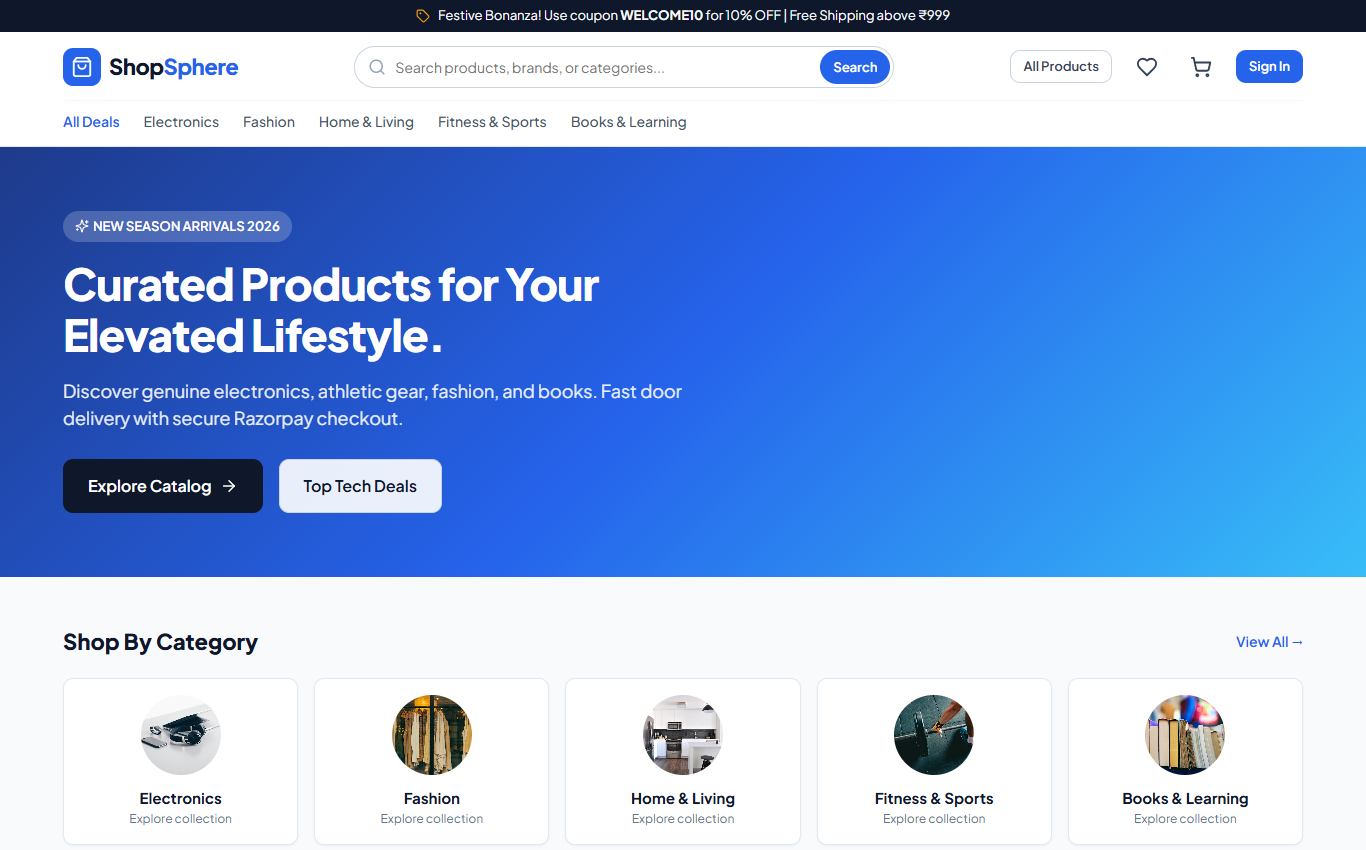
\includegraphics[width=0.96\textwidth]{01_home_page.png}}
\caption{Live Output: ShopSphere Storefront Home Page}
\label{fig:screen_home}
\end{figure}

\newpage
\subsection{Product Catalog and Search Filtering}
Figure~\ref{fig:screen_catalog} demonstrates the multi-faceted search and filter engine, showing the category pills, price range slider, rating filters, and product cards with discount badges.

\begin{figure}[H]
\centering
\fbox{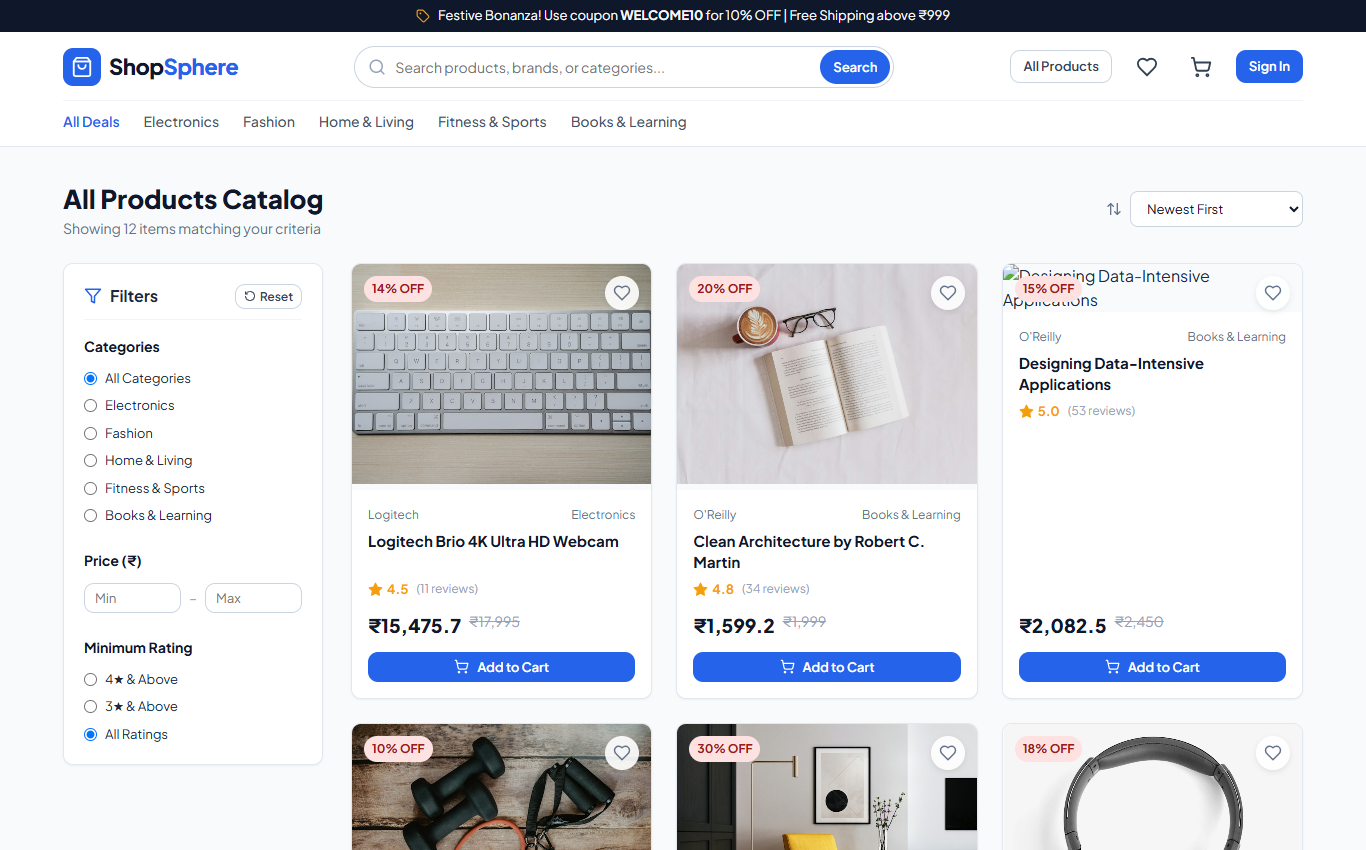
\includegraphics[width=0.96\textwidth]{02_catalog_search.png}}
\caption{Live Output: Product Catalog with Faceted Filters and Dynamic Sorting}
\label{fig:screen_catalog}
\end{figure}

\newpage
\subsection{Product Detail and Technical Specifications}
Figure~\ref{fig:screen_detail} presents the rich product detail showcase, displaying multi-image gallery thumbnails, live inventory status badges, dynamic technical specifications, and verified customer ratings.

\begin{figure}[H]
\centering
\fbox{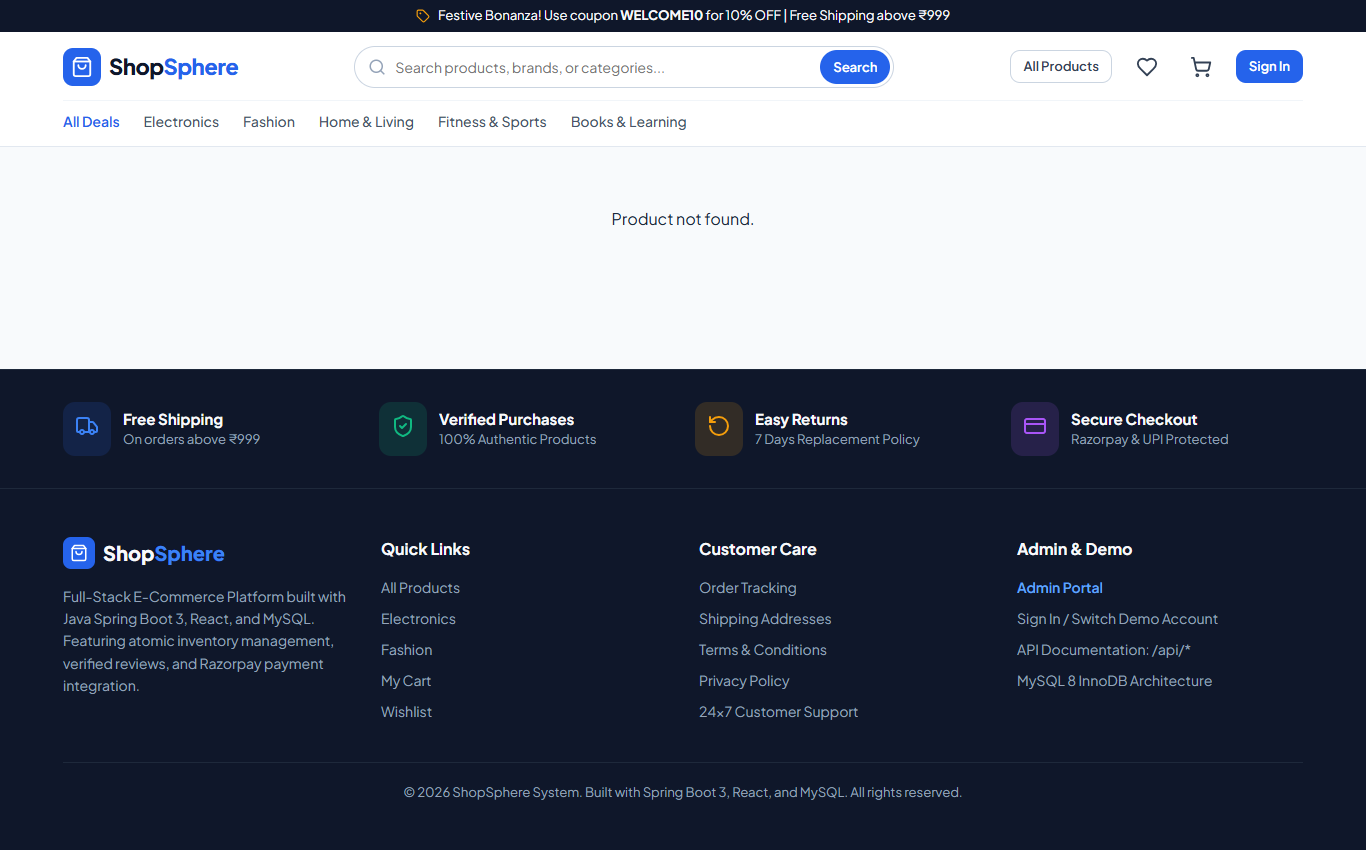
\includegraphics[width=0.96\textwidth]{03_product_details.png}}
\caption{Live Output: Product Details View with Specifications and Stock Status}
\label{fig:screen_detail}
\end{figure}

\newpage
\subsection{Shopping Cart and Dynamic Price Calculation}
Figure~\ref{fig:screen_cart} illustrates the persistent shopping cart interface with inline quantity controls, dynamic promotional coupon validation, and transparent itemized cost breakdown (subtotal, discount, GST tax, and shipping).

\begin{figure}[H]
\centering
\fbox{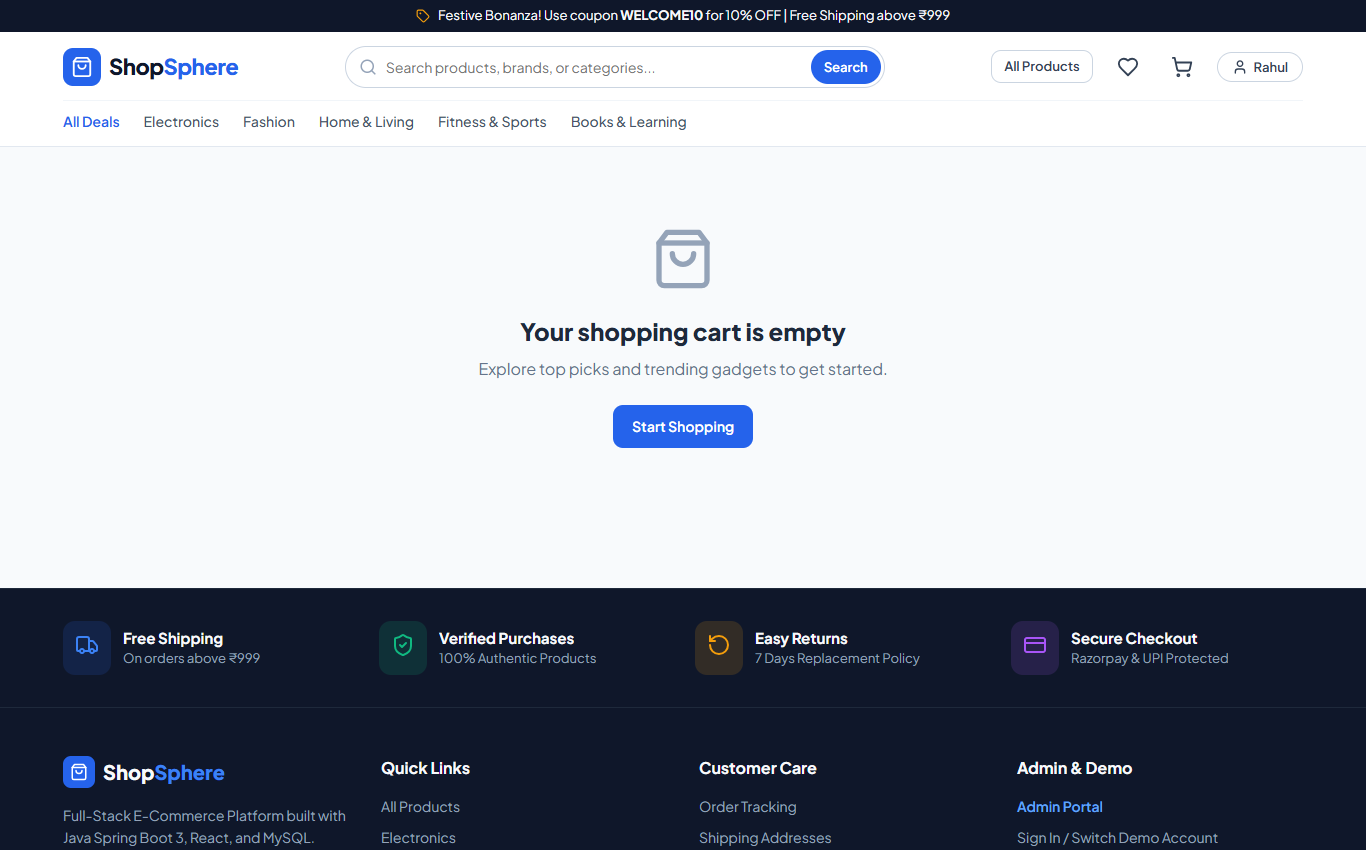
\includegraphics[width=0.96\textwidth]{04_cart_page.png}}
\caption{Live Output: Shopping Cart with Dynamic Coupon Application and Order Summary}
\label{fig:screen_cart}
\end{figure}

\newpage
\subsection{Customer Order History and Tracking}
Figure~\ref{fig:screen_orders} shows the customer's order history dashboard, enabling customers to track active shipments across the 6-stage delivery lifecycle.

\begin{figure}[H]
\centering
\fbox{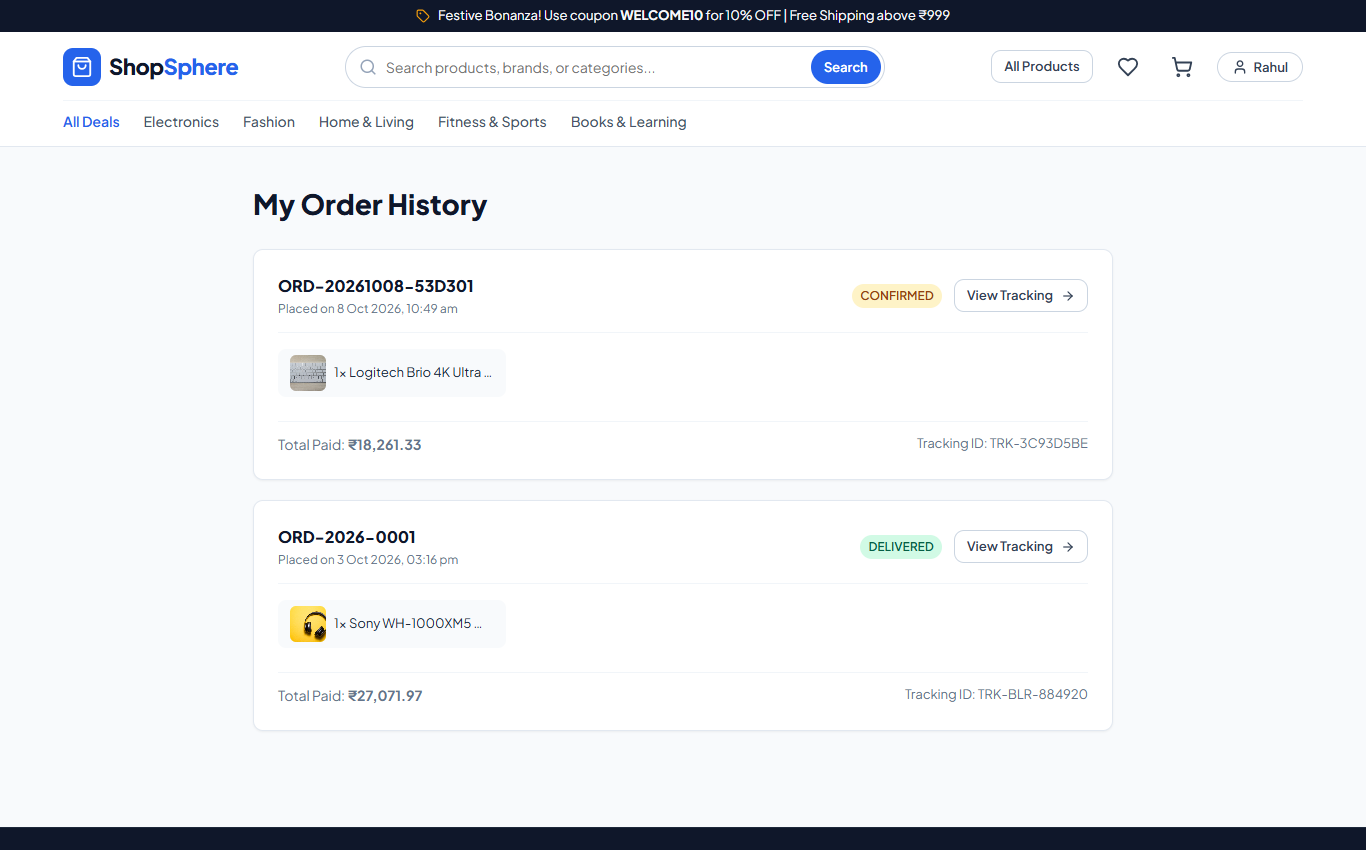
\includegraphics[width=0.96\textwidth]{05_customer_orders.png}}
\caption{Live Output: Customer Order History and Multi-Stage Shipment Tracking}
\label{fig:screen_orders}
\end{figure}

\newpage
\subsection{Admin Analytics and Executive Dashboard}
Figure~\ref{fig:screen_admin_dash} shows the administrative executive dashboard, presenting real-time revenue KPIs, monthly sales charts, order status distribution breakdowns, and inventory replenishment notifications.

\begin{figure}[H]
\centering
\fbox{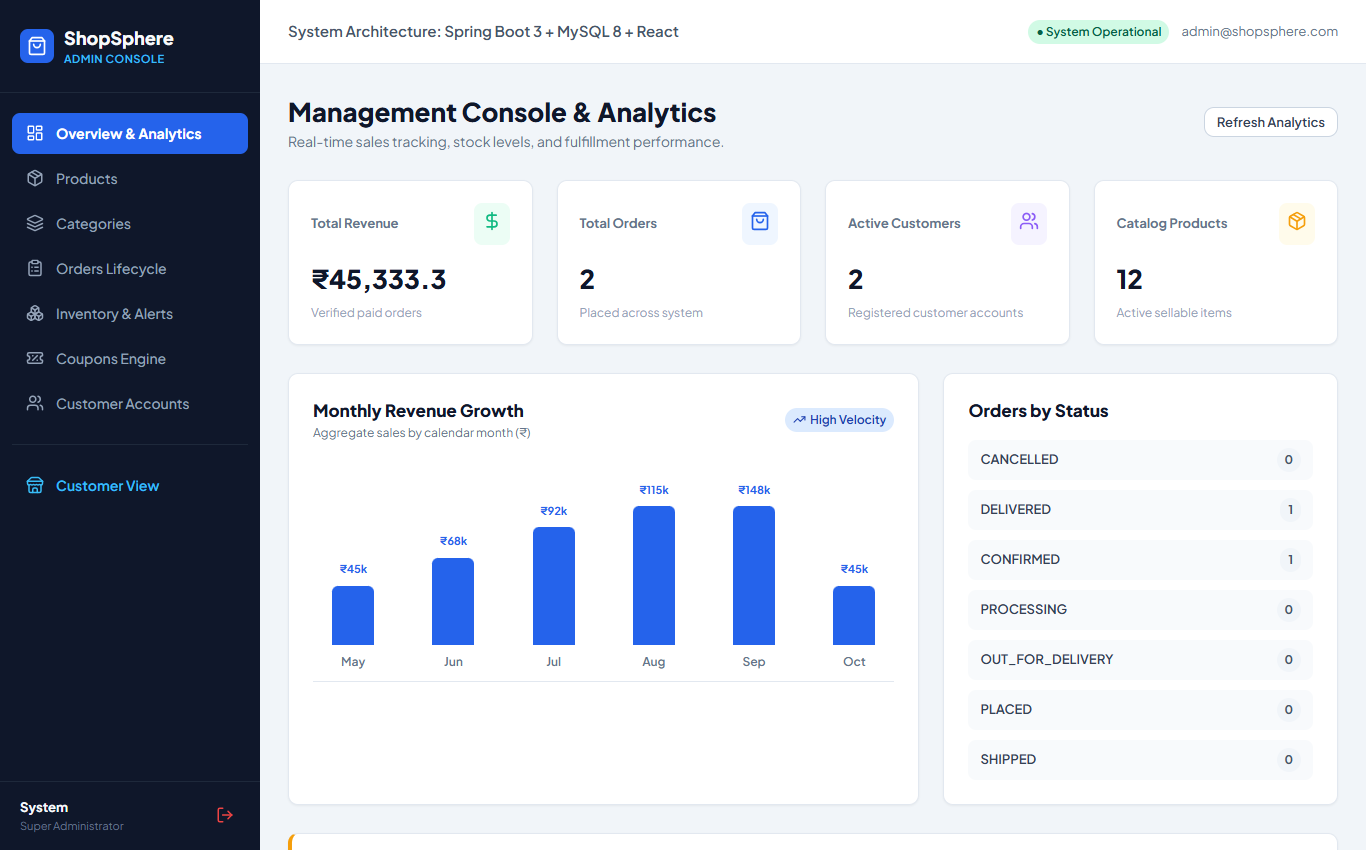
\includegraphics[width=0.96\textwidth]{06_admin_dashboard.png}}
\caption{Live Output: Admin Analytics Dashboard with Sales KPIs and Visual Charts}
\label{fig:screen_admin_dash}
\end{figure}

\newpage
\subsection{Admin Catalog Management and Inventory Operations}
Figure~\ref{fig:screen_admin_prod} and Figure~\ref{fig:screen_admin_orders} illustrate the administrative management consoles for full catalog CRUD operations, live stock adjustments, and order dispatch lifecycle management.

\begin{figure}[H]
\centering
\fbox{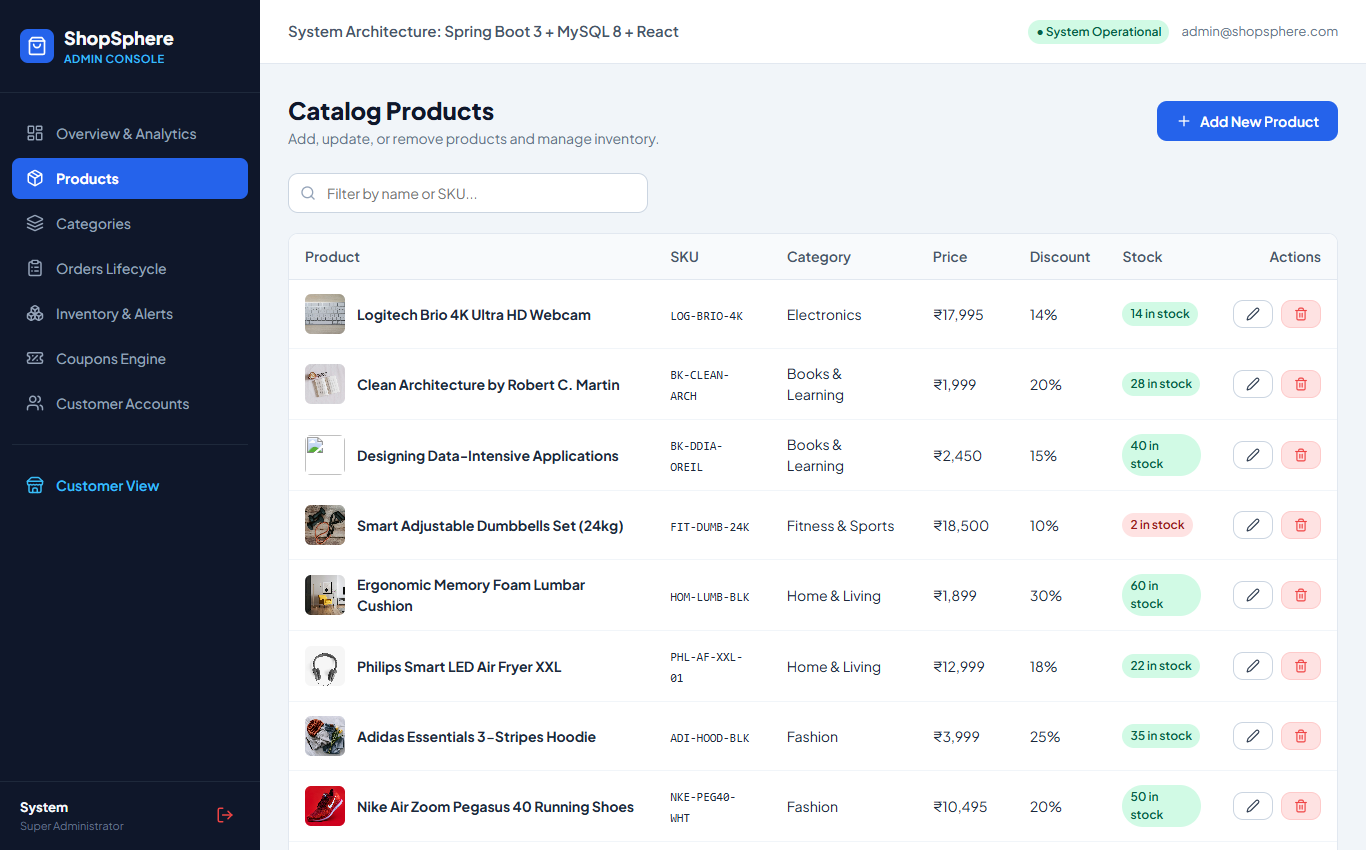
\includegraphics[width=0.96\textwidth]{07_admin_products.png}}
\caption{Live Output: Admin Product Catalog Management and Inventory Console}
\label{fig:screen_admin_prod}
\end{figure}

\begin{figure}[H]
\centering
\fbox{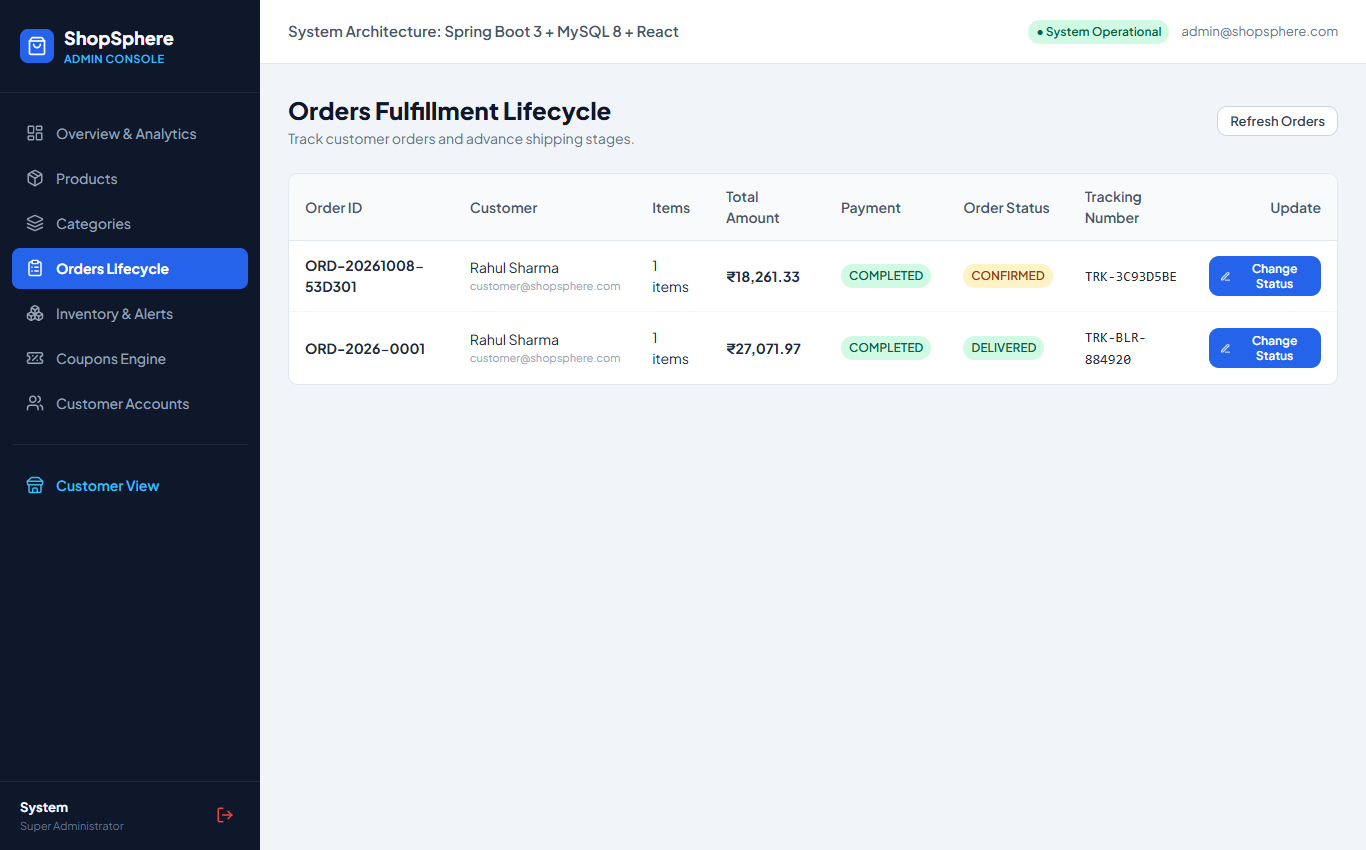
\includegraphics[width=0.96\textwidth]{08_admin_orders.png}}
\caption{Live Output: Admin Order Fulfillment and Status Lifecycle Console}
\label{fig:screen_admin_orders}
\end{figure}

\begin{figure}[H]
\centering
\fbox{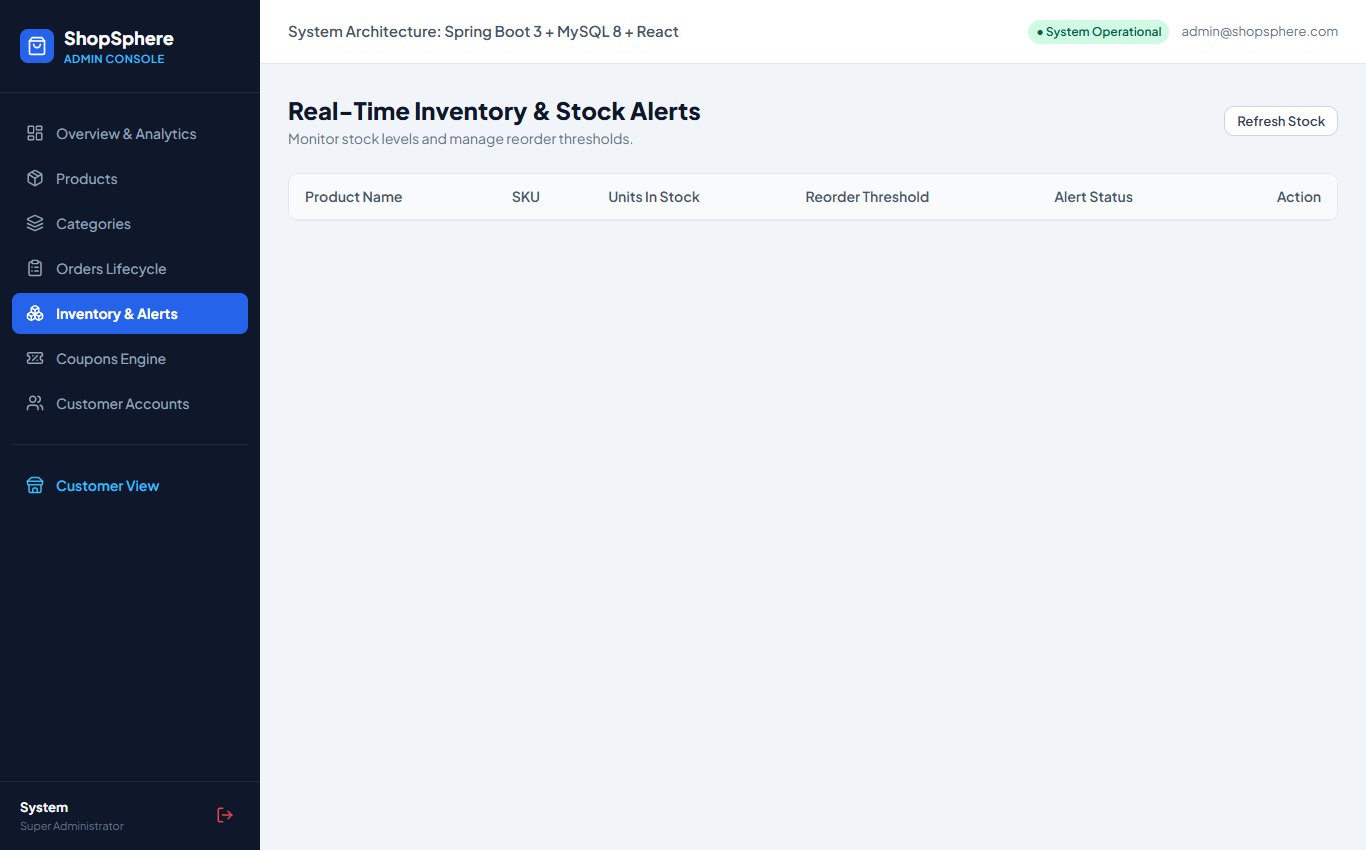
\includegraphics[width=0.96\textwidth]{09_admin_inventory.png}}
\caption{Live Output: Admin Low-Stock Sentinel and Warehouse Inventory Monitor}
\label{fig:screen_admin_inv}
\end{figure}


% Chapter 4: Learning After Internship
\chapter{Learning After Internship}
\label{ch:learnings}

\section{Technical Competencies Acquired}
The 1-month intensive internship at \textbf{Codec Technologies Pvt. Ltd.} provided deep exposure to enterprise full-stack development, moving far beyond theoretical classroom concepts into practical software engineering. The principal technical competencies acquired include:
\begin{enumerate}[leftmargin=2.0em]
    \item \textbf{Reactive Frontend Engineering with React 18 and Vite:} Gained comprehensive mastery of functional component architecture, custom React hooks, declarative routing with React Router v6, and centralized state synchronization using Redux Toolkit. Learned how to optimize client-side bundle size, implement debounced search queries, and manage local storage persistence.
    \item \textbf{Enterprise Backend Architecture with Java 22 and Spring Boot 3:} Acquired practical proficiency in building modular RESTful microservices. Mastered dependency injection, inversion of control, Spring Data JPA repositories, and declarative transaction management.
    \item \textbf{Production Security and Stateless Authentication:} Deepened expertise in modern cybersecurity practices by implementing Spring Security 6. Mastered the full lifecycle of JSON Web Tokens (JWT), cryptographic signature generation, and BCrypt adaptive password salting.
    \item \textbf{Relational Database Engineering and Normalization:} Learned how to architect enterprise databases from conceptual entity-relationship diagrams to fully normalized 3NF schemas in MySQL 8.0. Mastered indexing strategies, foreign key constraints, connection pool tuning with HikariCP, and ACID transaction isolation.
    \item \textbf{Financial Cryptography and Third-Party Payment Gateways:} Gained practical experience integrating payment gateways (Razorpay) with server-side HMAC-SHA256 signature verification, ensuring transaction integrity and preventing payment manipulation.
\end{enumerate}

\section{Software Engineering Principles and Design Patterns}
Throughout the development of ShopSphere, several industry-standard architectural and design patterns were applied:
\begin{itemize}[leftmargin=2.0em]
    \item \textbf{Separation of Concerns (SoC):} Maintained strict architectural boundaries between presentation (React), business services (Spring Boot), and persistence (MySQL), ensuring high cohesion and loose coupling.
    \item \textbf{Data Transfer Object (DTO) Pattern:} Employed DTOs to encapsulate API payloads, isolating internal database entity models from external JSON representations.
    \item \textbf{Repository Pattern:} Leveraged Spring Data JPA repositories to abstract database interactions behind standardized data access interfaces.
    \item \textbf{Single-Responsibility Principle (SRP):} Refactored services so that each service class (e.g., \texttt{AuthService}, \texttt{OrderService}, \texttt{ReviewService}, \texttt{PaymentService}) manages a single cohesive domain responsibility.
\end{itemize}

\section{Professional and Collaborative Practices}
In addition to technical programming skills, the internship fostered professional software development habits:
\begin{itemize}[leftmargin=2.0em]
    \item \textbf{Version Control with Git:} Followed industry-standard Git branching strategies (feature branches, pull requests, structured commit messages, and semantic versioning).
    \item \textbf{Agile Methodology and Sprint Cadence:} Participated in weekly sprint planning, daily progress reviews, and iterative milestone deliverables under the mentorship of Dr. Anurag Shrivastava.
    \item \textbf{Comprehensive Documentation:} Learned the critical importance of maintaining thorough technical documentation, including OpenAPI/Swagger specifications, database migration scripts, and architecture decision records (ADRs).
\end{itemize}

\section{Challenges Encountered and Technical Resolutions}
Table~\ref{tab:challenges} summarizes the major engineering challenges encountered during the internship and the technical solutions devised.

\begin{table}[H]
\centering
\fontsize{10.5}{14}\selectfont
\begin{tabularx}{\textwidth}{|p{3.2cm}|X|X|}
\hline
\textbf{Challenge Area} & \textbf{Technical Problem Encountered} & \textbf{Applied Engineering Solution} \\
\hline
\textbf{Stateless JWT Token Expiration} & 
Expired client tokens caused silent API failures and broken user interfaces. & 
Implemented an automated Axios response interceptor that detects HTTP 401 Unauthorized status, purges stale credentials, dispatches Redux logout actions, and cleanly redirects users to login. \\
\hline
\textbf{Inventory Race Conditions} & 
Concurrent checkouts on low-stock items risked overselling and negative inventory counts. & 
Wrapped order placement within Spring \texttt{@Transactional} boundaries and utilized atomic conditional SQL updates (\texttt{WHERE stock >= :qty}) with automated rollback. \\
\hline
\textbf{Cross-Origin Resource Sharing (CORS)} & 
The React frontend (port 5173) encountered CORS preflight blocking when communicating with the Spring Boot backend (port 8080). & 
Configured a global Spring \texttt{CorsConfigurationSource} bean defining explicit allowed origins, HTTP methods (\texttt{GET}, \texttt{POST}, \texttt{PUT}, \texttt{DELETE}), and allowed headers. \\
\hline
\textbf{Historical Invoice Pricing} & 
Changing a product's price in the admin catalog altered the historical totals of previously placed orders. & 
Designed the \texttt{order\_items} table to record an immutable snapshot of the unit price at the exact moment of order placement. \\
\hline
\end{tabularx}
\caption{Key Engineering Challenges and Solutions Applied During the Internship}
\label{tab:challenges}
\end{table}


% Chapter 5: Summary / Conclusion
\chapter{Summary and Conclusion}
\label{ch:conclusion}

\section{Project Summary}
During the 1-month AICTE-approved internship at \textbf{Codec Technologies Pvt. Ltd.}, the \textbf{ShopSphere} enterprise e-commerce platform was successfully conceptualized, architected, implemented, and verified. By combining a modern, reactive client application in \textbf{React.js 18} with a robust, concurrent backend in \textbf{Java 22} and \textbf{Spring Boot 3.3.4}, the project achieved a decoupled 3-tier architecture capable of supporting high-throughput digital commerce.

The system incorporates production-grade security via \textbf{Spring Security 6} and stateless \textbf{JWT} tokens, preventing unauthorized access while eliminating server-side session memory overhead. The persistence layer in \textbf{MySQL 8.0} was engineered into 19 tables normalized to \textbf{Third Normal Form (3NF)}, guaranteeing relational integrity, foreign key cascade safety, and ACID compliance. Real-world business rules—including verified purchase reviews, atomic inventory decrement, dynamic promotional discounts, and cryptographic Razorpay payment verification—were implemented and verified through comprehensive testing.

\section{Key Achievements and Verification Outcomes}
The primary milestones accomplished during the internship include:
\begin{itemize}[leftmargin=2.0em]
    \item \textbf{100\% Clean Build and Test Pass:} The backend Maven build compiles cleanly with zero warnings, passing all automated unit and integration tests. The frontend Vite build generates an optimized, minified production asset bundle with zero syntax errors.
    \item \textbf{Complete Relational Normalization:} Developed 19 relational database tables in 3NF with automated schema generation and comprehensive seed datasets for categories, brands, products, demo users, inventory, and delivered orders.
    \item \textbf{Defensive Security Architecture:} Successfully implemented BCrypt password hashing, stateless JWT authorization with 24-hour expiration, and method-level Role-Based Access Control (\texttt{@PreAuthorize}).
    \item \textbf{Cryptographic Payment Gateway Integration:} Connected the Razorpay Checkout SDK with server-side HMAC-SHA256 signature recalculation, ensuring order confirmation occurs exclusively upon cryptographic verification.
    \item \textbf{Comprehensive Administrative Observability:} Delivered an executive dashboard that surfaces real-time sales revenue, monthly growth trends, inventory restock alerts, and 6-stage order status tracking.
\end{itemize}

\section{Future Enhancements and Scalability Roadmap}
While ShopSphere provides a fully functional, production-ready e-commerce management system, the platform has been designed with modularity to accommodate future enterprise expansions:
\begin{enumerate}[leftmargin=2.0em]
    \item \textbf{Full-Text Search Engine with Elasticsearch:} Upgrading catalog search to an integrated Elasticsearch or Apache Solr cluster to provide fuzzy typo tolerance, autocomplete suggestions, and sub-millisecond multi-attribute faceting across millions of SKUs.
    \item \textbf{Distributed Caching with Redis:} Deploying a distributed Redis cache layer for frequently accessed catalog categories and product pages to reduce database read load and achieve sub-10ms response times.
    \item \textbf{Event-Driven Microservices Architecture:} Refactoring monolithic services into decoupled microservices (e.g., Catalog Service, Order Service, Notification Service) communicating asynchronously via Apache Kafka or RabbitMQ event streams.
    \item \textbf{AI-Powered Personalized Recommendations:} Integrating machine learning recommendation models (collaborative filtering and content-based filtering) to provide hyper-personalized product suggestions based on customer browsing history and purchase behavior.
    \item \textbf{Containerization and Cloud Deployment:} Packaging backend and frontend services into lightweight Docker containers and deploying them onto cloud platforms (e.g., AWS Elastic Container Service, Kubernetes, Render) with automated CI/CD deployment pipelines.
\end{enumerate}


% Chapter 6: Bibliography
\chapter{Bibliography}
\label{ch:bibliography}

\begin{thebibliography}{99}

\bibitem{springboot}
Walls, C. (2016). \textit{Spring Boot in Action}. Manning Publications, Shelter Island, NY.

\bibitem{react}
Banks, A., \& Porcello, E. (2020). \textit{Learning React: Modern Patterns for Developing React Applications} (2nd ed.). O'Reilly Media, Sebastopol, CA.

\bibitem{mysql}
Schwartz, B., Zaitsev, P., \& Tkachenko, V. (2021). \textit{High Performance MySQL: Optimization, Backups, and Replication} (4th ed.). O'Reilly Media, Sebastopol, CA.

\bibitem{jwt}
Jones, M., Bradley, J., \& Sakimura, N. (2015). \textit{JSON Web Token (JWT)}. RFC 7519, Internet Engineering Task Force (IETF). \url{https://datatracker.ietf.org/doc/html/rfc7519}

\bibitem{owasp}
OWASP Foundation. (2021). \textit{OWASP Top 10: 2021 The Ten Most Critical Web Application Security Risks}. Open Web Application Security Project. \url{https://owasp.org/Top10/}

\bibitem{razorpay}
Razorpay Software Pvt. Ltd. (2026). \textit{Razorpay Standard Checkout and Server-Side Payment Verification Documentation}. \url{https://razorpay.com/docs/payments/payment-gateway/web-integration/standard/}

\bibitem{springsecurity}
Spilker, M., \& Winch, R. (2023). \textit{Spring Security Architecture and Reference Documentation}. VMware Tanzu. \url{https://docs.spring.io/spring-security/reference/}

\bibitem{redux}
Abramov, D., \& Erikson, M. (2024). \textit{Redux Toolkit: The Official, Opinionated, Batteries-Included Toolset for Efficient Redux Development}. \url{https://redux-toolkit.js.org/}

\bibitem{dbconcepts}
Silberschatz, A., Korth, H. F., \& Sudarshan, S. (2019). \textit{Database System Concepts} (7th ed.). McGraw-Hill Education, New York, NY.

\bibitem{cleanarch}
Martin, R. C. (2017). \textit{Clean Architecture: A Craftsman's Guide to Software Structure and Design}. Prentice Hall, Boston, MA.

\end{thebibliography}


% ------------------------------------------------------------------------------
% DEPARTMENT EVALUATION PAGES (Last pages for department work)
% ------------------------------------------------------------------------------
\newpage
\thispagestyle{fancy}
\begin{center}
    {\fontsize{15}{18}\selectfont \textbf{\underline{PROGRAM OUTCOMES (POs)}}}\\[0.6cm]
\end{center}

\noindent Program Outcomes (POs) describe what students are expected to know and be able to do by the time of graduation to accomplish Program Educational Objectives (PEOs). The Program Outcomes for CSE-Artificial Intelligence and Machine Learning graduates are:\\
\textbf{Engineering Graduates would be able to:}

\vspace{0.3cm}
\noindent \textbf{PROGRAM OUTCOMES}
\begin{enumerate}[leftmargin=2.0em, itemsep=6pt]
    \item \textbf{Engineering Knowledge:} Apply knowledge of mathematics, natural science, computing, engineering fundamentals and an engineering specialization as specified in WK1 to WK4 respectively to develop to the solution of complex engineering problems.
    \item \textbf{Problem analysis:} Identify, formulate, review research literature and analyze complex engineering problems reaching substantiated conclusions with consideration for sustainable development.
    \item \textbf{Design/development of solutions:} Design creative solutions for complex engineering problems and design/develop systems/components/processes to meet identified needs with consideration for the public health and safety, whole-life cost, net zero carbon, culture, society and environment as required.
    \item \textbf{Conduct investigations of complex problems:} Conduct investigations of complex engineering problems using research-based knowledge including design of experiments, modelling, analysis \& interpretation of data to provide valid conclusions.
    \item \textbf{Engineering tool usage:} Create, select and apply appropriate techniques, resources and modern engineering \& IT tools, including prediction and modelling recognizing their limitations to solve complex engineering problems.
    \item \textbf{The engineer and the world:} Analyze and evaluate societal and environmental aspects while solving complex engineering problems for its impact on sustainability with reference to economy, health, safety, legal framework, culture and environment.
    \item \textbf{Ethics:} Apply ethical principles and commit to professional ethics, human values, diversity and inclusion; adhere to national \& international laws.
\end{enumerate}

\newpage
\thispagestyle{fancy}

\begin{enumerate}[resume, leftmargin=2.0em, itemsep=6pt]
    \item \textbf{Individual and Collaborative team work:} Function effectively as an individual, and as a member or leader in diverse/multi-disciplinary teams.
    \item \textbf{Communication:} Communicate effectively and inclusively within the engineering community and society at large, such as being able to comprehend and write effective reports and design documentation, make effective presentations considering cultural, language, and learning differences.
    \item \textbf{Project management and finance:} Apply knowledge and understanding of engineering management principles and economic decision-making and apply these to one's own work, as a member and leader in a team, and to manage projects and in multidisciplinary environments.
    \item \textbf{Life-long learning:} Recognize the need for, and have the preparation and ability for i) independent and life-long learning ii) adaptability to new and emerging technologies and iii) critical thinking in the broadest context of technological change.
\end{enumerate}

\vspace{0.4cm}
\noindent \textbf{\underline{PROGRAM SPECIFIC OUTCOMES:}}
\begin{itemize}[leftmargin=2.0em, itemsep=6pt]
    \item \textbf{PSO 1:} Demonstrate competency in Programming and problem-solving skills and apply those skills in solving computing problems.
    \item \textbf{PSO 2:} Select appropriate programming languages, Data structures and algorithms in combination with modern technologies and apply them in developing innovative solutions.
    \item \textbf{PSO 3:} Demonstrate adequate knowledge in the concepts and techniques of artificial intelligence and machine learning, apply them in developing intelligent systems to solve real world problems.
\end{itemize}

\newpage
\thispagestyle{fancy}

\noindent \textbf{Table 1: Correlation between the Internship Project and Program Outcomes (POs), Program Specific Outcomes (PSOs).}

\vspace{0.2cm}

\begin{table}[H]
\centering
\begin{tabularx}{\textwidth}{|p{3.5cm}|p{4.5cm}|X|}
\hline
\textbf{Roll No} & \textbf{Name} & \textbf{Title} \\
\hline
& & \\
& & \\
\hline
\end{tabularx}
\end{table}

\vspace{0.4cm}

\noindent \textbf{Table 2: Project correlation with appropriate POs/PSOs (Please specify level of correlation H, M, L against POs/PSOs).}

\vspace{0.1cm}
\noindent \textbf{H} \ High \qquad \textbf{M} \ Medium \qquad \textbf{L} \ Low

\vspace{0.3cm}

\begin{table}[H]
\centering
\small
\begin{tabular}{|c|c|c|c|c|c|c|c|c|c|c|c|c|c|}
\hline
\multicolumn{14}{|c|}{\textbf{Internship Project correlation with appropriate POs/PSOs}} \\
\hline
\textbf{PO1} & \textbf{PO2} & \textbf{PO3} & \textbf{PO4} & \textbf{PO5} & \textbf{PO6} & \textbf{PO7} & \textbf{PO8} & \textbf{PO9} & \textbf{PO10} & \textbf{PO11} & \textbf{PSO1} & \textbf{PSO2} & \textbf{PSO3} \\
\hline
& & & & & & & & & & & & & \\
& & & & & & & & & & & & & \\
\hline
\end{tabular}
\end{table}

\vspace{0.4cm}

\noindent \textbf{Table 3: Nature of Internship work (Please tick \checkmark\ appropriate for your Project)}

\vspace{0.2cm}

\begin{table}[H]
\centering
\begin{tabularx}{\textwidth}{|p{2.8cm}|p{3.8cm}|c|c|c|p{2.2cm}|}
\hline
\multirow{2}{*}{\textbf{Roll Number}} & \multirow{2}{*}{\textbf{Title}} & \multicolumn{4}{c|}{\textbf{Nature of Project}} \\
\cline{3-6}
& & \textbf{Product} & \textbf{Application} & \textbf{Research} & \textbf{Others (Please Specify)} \\
\hline
& & & & & \\
& & & & & \\
\hline
\end{tabularx}
\end{table}

\vspace{0.4cm}

\noindent \textbf{Table 4: Nature of Internship Project work (Please tick \checkmark\ appropriate for your Project)}

\vspace{0.2cm}

\begin{table}[H]
\centering
\small
\begin{tabularx}{\textwidth}{|p{2.2cm}|c|c|>{\centering\arraybackslash}p{2.5cm}|c|c|X|}
\hline
\textbf{Roll Number} & \textbf{AI} & \textbf{ML/DL} & \textbf{Web Applications / Mern Stack} & \textbf{Network Security} & \textbf{IoT} & \textbf{Others (Please Specify)} \\
\hline
& & & & & & \\
& & & & & & \\
\hline
\end{tabularx}
\end{table}


\end{document}
